%% $RCSfile: proj_report_outline.tex,v $
%% $Revision: 1.3 $
%% $Date: 2016/06/10 03:41:54 $
%% $Author: kevin $




\documentclass[11pt
              , a4paper
              , twoside
              , openright
              ]{report}


\usepackage{pdfpages}
\usepackage{amsmath}
\usepackage{amssymb}
\usepackage{graphicx}
\usepackage{bm}
\usepackage{subcaption}
\usepackage{float} % lets you have non-floating floats
\usepackage{booktabs}
\usepackage{url} % for typesetting urls
\usepackage{siunitx}
\usepackage{cleveref}


%
%  We don't want figures to float so we define
%
\newfloat{fig}{thp}{lof}[chapter]
\floatname{fig}{Figure}

%% These are standard LaTeX definitions for the document
%%                            
\title{Bayesian estimation of bound fluid fraction from NMR relaxation \\ Final Report}
\author{David Dobbie}

%% This file can be used for creating a wide range of reports
%%  across various Schools
%%
%% Set up some things, mostly for the front page, for your specific document
%
% Current options are:
% [ecs|msor|sms]          Which school you are in.
%                         (msor option retained for reproducing old data)
% [bschonscomp|mcompsci]  Which degree you are doing
%                          You can also specify any other degree by name
%                          (see below)
% [font|image]            Use a font or an image for the VUW logo
%                          The font option will only work on ECS systems
%
\usepackage[image,ecs,]{vuwproject}
%\usepackage[a4paper]{geometry}
% You should specifiy your supervisor here with
     \supervisors{Paul Teal, Robin Dykstra}
% use \supervisors if there is more than one supervisor

% Unless you've used the bschonscomp or mcompsci
%  options above use
   \otherdegree{Bachelor of Engineering with Honours in Electronic and Computer Systems Engineering}
% here to specify degree

% Comment this out if you want the date printed.
\date{}

\begin{document}

% Make the page numbering roman, until after the contents, etc.
\frontmatter

%%%%%%%%%%%%%%%%%%%%%%%%%%%%%%%%%%%%%%%%%%%%%%%%%%%%%%%

%%%%%%%%%%%%%%%%%%%%%%%%%%%%%%%%%%%%%%%%%%%%%%%%%%%%%%%

\begin{abstract}

Effective measurements of NMR relaxation have typically been constrained to high SNR environments due to the adverse effect that noise can have. Inversion of the measured data to its relaxation density function is an ill-posed problem. The current literature has worked on increasing the accuracy of inversion given only measured data and the nature of the noise. These techniques have been recreated and bench marked in this report. This project seeks to use Bayesian techniques to integrate prior data based on high quality measurements in order to make more accurate inversions of  measured data. This is used to compute the bound fluid fraction of porous  media to assess the difficulty of fluid extraction.
\end{abstract}

%%%%%%%%%%%%%%%%%%%%%%%%%%%%%%%%%%%%%%%%%%%%%%%%%%%%%%%

\maketitle

\tableofcontents

% we want a list of the figures we defined
%\listof{fig}{Figures}

%%%%%%%%%%%%%%%%%%%%%%%%%%%%%%%%%%%%%%%%%%%%%%%%%%%%%%%

\mainmatter

%%%%%%%%%%%%%%%%%%%%%%%%%%%%%%%%%%%%%%%%%%%%%%%%%%%%%%%

% individual chapters included here


\chapter{Introduction}\label{C:intro}
Relaxation times gathered from nuclear magnetic resonance (NMR) experiments provide insight into the physical nature of a sample \cite{GruberLinearFunctionals2013}. However, most NMR experiments are restricted to a limited environment - like a laboratory \cite{IntrinsicSNREdelstein1986}. To be practicable in use cases that have constraints such as high noise or low signal power, more advanced signal processing is required. This preliminary report details the progress made in developing a new technique of extending the use to NMR to nosier environments. The focus is on a specific attribute: the bound fluid fraction of porous media.
\section{Motivation}
The motivation of this project is to improve upon traditional techniques of gathering relaxation times from measured data gathered in low signal-to-noise ratio (SNR) environments. Development of this technology has originally been focused on the goal of testing the viability of oil wells \cite{wellLoggingBook}. The specific goal was to estimate how easy it was to extract fluid out of the rock at an extraction point. Often this is a very high noise environment that is poorly controlled, necessitating the use of robust estimation techniques \cite{BadTruthLaplaceEpstein2008} \cite{NumericalInversionLaplaceTransform1978}. An improvement in NMR processing can be translated to other use cases where the power is limited. These can include identifying the nature of fluids in food products \cite{NMRFOODCapitani2017}.
\section{Aim}
The aims of this project are to:
\begin{enumerate}
    \item Implement and evaluate the competing techniques for finding distributions of T2 relaxation times.
    \item Implement and evaluate new techniques using Bayesian statistics to establish the distribution of T2 relaxation times.
    \item Use these techniques to improve upon the estimation of the bound fluid fraction of a sample.
\end{enumerate}


\section{Proposal Review}
Compared to the initial proposal, the project is closely aligned with the goals and scope outlined in it. As the project up to this point has been focused on implementing the competing algorithms there has been minimal scope drift. The problem being solved is well understood in the literature and has a goal that can be numerically validated. 


The main change from the proposal was to add more focus onto bound fluid fraction ($BFF$) detected in a sample. This is a numerical value that allows for a non-trivial insight into the sample being measured. The density function of T2 relaxation times is an important intermediate step to the $BFF$. However, the density function provides more information than is needed in many physical use cases. The addition of this aim to the project more closely meets its scope to tangible and directly application.

 


\chapter{Background}\label{C:back}
Processing NMR relaxation in low SNR environments is crucial for dynamic environments such as well logging \cite{wellLoggingBook} \cite{UsingNMRPetrophysicalKenyon1992nuclear}. The previously published work forms the benchmark for comparison with this project's proposed technique. This background survey details the current published technique, the evaluation criteria of the techniques, and the Bayesian theory that informs the design in Chapter \ref{C:design}.

\section{NMR Relaxation}
Nuclear magnetic resonance involves determining the nature of the nuclei of a sample by using its magnetic behaviour \cite{NMRSignalProcessingBook}. To provide an effective basis for the signal processing techniques to operate on, we start by examining the physics of the magnetism of the nuclei.



\subsection{Underlying Physics}

\subsubsection{Magnetism of the Nuclei}
The nucleus has two classical aspects that make it a microscopic magnet \cite{NMRSignalProcessingBook}:
\begin{enumerate}
    \item a nucleus has an electrical charge from the protons that make it up, and
    \item it may have a non-zero spin.
\end{enumerate}
The spin creates a magnetic dipole moment, $\vec{\mu}$. This phenomenon is expressed as the relation of angular momentum $\vec{J}$ and the gyro-magnetic ratio inherent to the nuclei, $\gamma$, such that

\begin{equation}
    \vec{\mu} = \gamma \vec{J}
    \label{eq:magneticMomentEquation}
\end{equation}
A macroscopic magnetic field formed by many nuclei, $\vec{M}$, is the summation over the total number of spins in the system, $N_s$  \cite{NMRSignalProcessingBook}.

\begin{equation}
    \vec{M} = \sum^{N_s}_{n = 1}\vec{\mu_{n}}
    \label{eq:macroMagnetic}
\end{equation}

Introducing a static magnetic field $B_0$ induces rotation of the magnetic moments of the nuclei. This rotation about the axis of $B_0$ is called nuclear precession. The angular frequency of this rotation is known as the Larmor frequency  \cite{NMRSignalProcessingBook}. This is given by: 
\begin{equation}
    \omega_0 = \gamma B_0
    \label{ref:LarmorFreq}
\end{equation}
Holding the magnetic field $B_0$ constant means that all the same nuclei exhibit nuclear precession at the same frequency. Their magnetic dipoles precess at the same frequency.

In order to set all of the rotations of magnetic dipoles into the same phase we require another magnetic field, $B_1$. This field makes the system phase coherent  \cite{NMRSignalProcessingBook}. This is so that all of the magnetic dipoles of the same frequency constructively interfere, providing a strong enough signal to measure. $B_1$ is in the form of a short RF (radio frequency) pulse that lasts from microseconds to the milliseconds  \cite{NMRSignalProcessingBook}.

With phase coherence achieved there is a measurable macroscopic magnetic field originating from the nuclei. The change of this nuclei magnetic field is described by the Bloch Equation  \cite{NMRSignalProcessingBook}:
\begin{equation}
    \frac{d\vec{M}}{dt} = \gamma \vec{M} \times \vec{B} - \frac{M_{x}\vec{i} + M_{y}\vec{j}}{T_2} - \frac{(M_z - M_{z}^0)\vec{k}}{T_1}
    \label{eq:blochEquation}
\end{equation}
where $\vec{M} = (M_x, M_y, M_z)$.
\subsubsection{Relaxation}

At the end of an RF pulse, the magnetic field $B_1$ is set to 0  \cite{NMRSignalProcessingBook}. In the rotating frame of reference this eliminates the first term of the Bloch equation. This results in the magnetism of the system of nuclei to be described by two differential equations:
\begin{equation}
    \begin{cases}
          \frac{dM_{z'}}{dt}    =         -\frac{M_{z'} - M_{z}^0}{T_1}  \\
           \frac{dM_{x'y'}}{dt}    =         -\frac{M_{x'y'}}{T_2}  \\         
    \end{cases}
\end{equation}
The time evolution of the system is governed by these equations. Immediately after the RF pulse ($t = 0_+$) for the transverse magnetic field, $M_{x'y'}$, is expressed as:

\begin{equation}
    M_{x'y'}(t) = M_{x'y'}(0_+) e^{-t/T_2}
    \label{eq:T2ExpoenetialRelaxation}
\end{equation}

This exponential decay is referred to as the $T_2$ relaxation  \cite{NMRSignalProcessingBook}. The decay constant $T_2$ is used to give insight to the physical properties of the nuclei in the sample. This exponential model is only suitable for weak spin-spin systems such as fluids. Therefore, the analysis of the $T_2$ relaxation is limited to the behaviour of the fluids in a sample.

\subsubsection{Detecting Relaxation}
The resultant magnetic field can be detected by using Faraday's Law and the principle of reciprocity \cite{NMRSignalProcessingBook}:

\begin{equation}
    V(t) = -\frac{\partial \Phi(t)}{\partial t} = - \frac{\partial}{\partial t} \int_\text{object} \vec{B_r}(\bm{r}) \cdot \vec{M}(\bm{r} \cdot t) d \bm{r}
    \label{eq:detectionFaraday}
\end{equation}

$\vec{B_r}(\bm{r})$ is the magnetic field produced by the coil by a hypothetical unit direct current. After demodulation of the voltage \cite{NMRSignalProcessingBook}, we get a measurement signal we can process and analyse:

\begin{equation}
    m(t) = \int_{\text{object}} M_{x,y}(\bm{r}, 0 )e^{i\gamma \Delta B(\bm{r})t} d \bm{r}
    \label{eq:detectionFinalSignal}
\end{equation}
The term $\Delta B $ varies in space due to the inhomogeneity of the magnetic field. This is a form of error introduced into the measurement process, which is more pronounced in field measurement tools rather than in laboratory tools. Figure \ref{fig:example_field_tool} illustrates an example field measurement tool and its grossly inhomogeneous magnetic field.

\begin{figure}[htb]
    \centering
    \includegraphics[width=0.75\textwidth]{backgroundImages/example_of_tool}
    \caption{An example of a field measurement tool used to detect relaxation for the rock in a bore hole \cite{nmr_picture_tool}}.
    \label{fig:example_field_tool}
\end{figure}



\subsection{The $T_2$ Density Function}
The density function of T2 relaxation times is denoted by $f(T_2)$. An example $T_2$ distribution is shown in Figure \ref{fig:theModel}. The T2 density function forms the basis of analysis of fluids in a sample. There are several properties that relate T2 relaxation to fluids in porous media. The most significant two we shall analyse are: \textit{porosity}, and \textit{bound fluid fraction} \cite{NMRForRockskleinberg1993nuclear} \cite{wellLoggingBook}.

\begin{figure} [h]
    \centering
    \begin{subfigure}[b]{0.495\textwidth}
        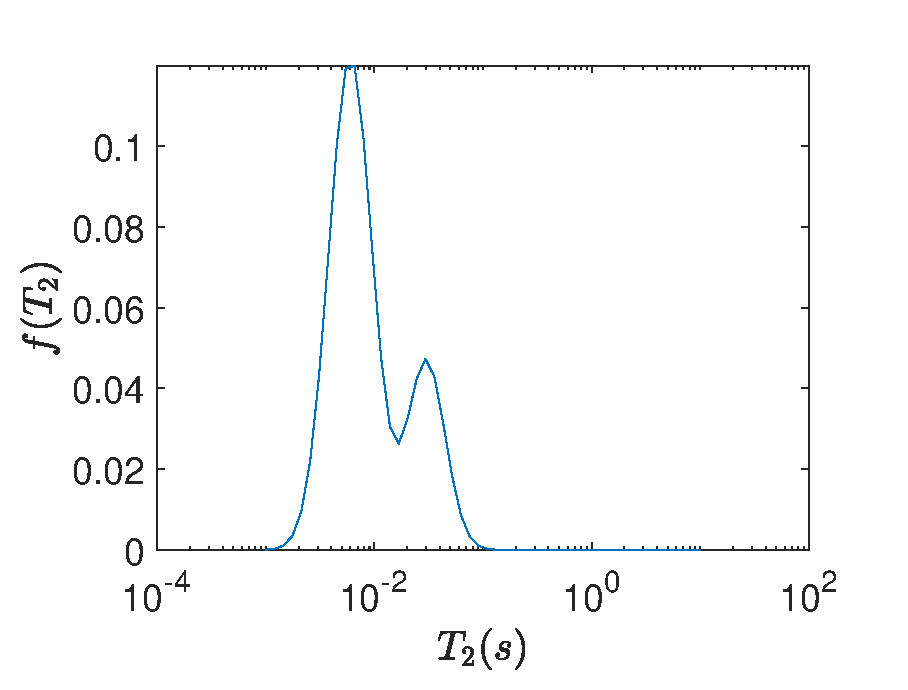
\includegraphics[width=\textwidth]{backgroundVector/densityFunction.eps}
        \subcaption{The density function $f(T_2)$}
        \label{fig:densityFunction}
    \end{subfigure}
    \begin{subfigure}[b]{0.495\textwidth}
        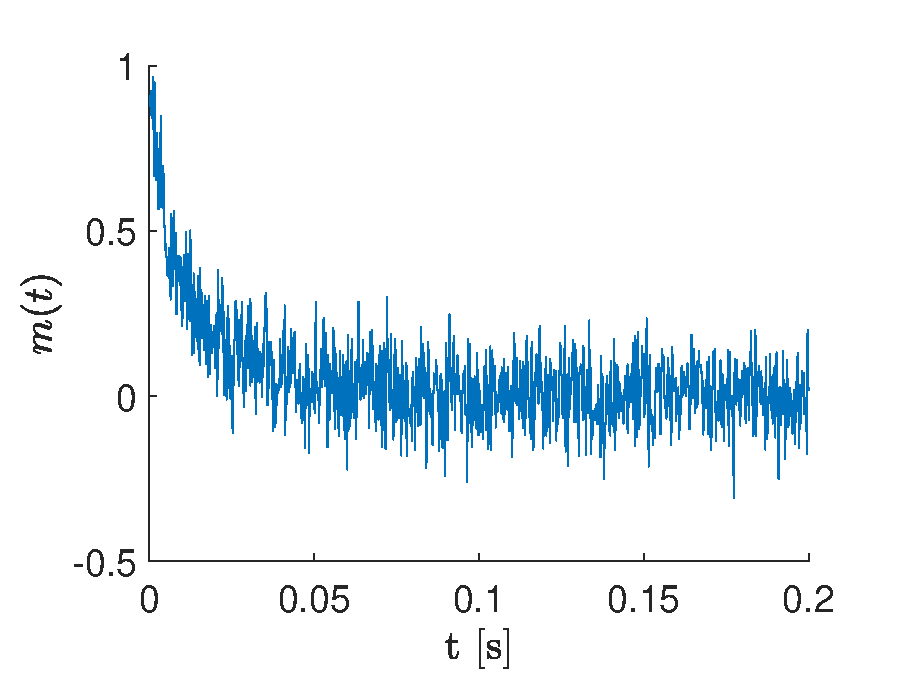
\includegraphics[width=\textwidth]{backgroundVector/measured.eps}
        \subcaption{The modelled measured data $m(t)$}
        \label{fig:measuredData}
    \end{subfigure}
    
    \caption{An example modelled $T_2$ density function and the measured data generated from it. It has unity porosity and a noise standard deviation of $\sigma_\epsilon = 0.2$}
    \label{fig:theModel}
\end{figure}

\subsubsection{Porosity}
The fraction of the rock volume that can be occupied by fluid is defined as the porosity ($\phi$) \cite{PorosityandT2Times}. After calibration with a water sample ($\phi = 1$), the integral over the entire density function is equal to the porosity.
\begin{equation}
    \label{eq:porosity_defn}
    \phi = \int_0^\infty f(T_{2}) dT_{2}
\end{equation}
This is approximated by taking the sum over the discretised density function:
\begin{equation}
    \phi \approx \sum_i f(T_{2 i})
\end{equation}

\subsubsection{Bound Fluid Fraction}
Bound fluids are fluids that require significant capillary pressure to remove from porous media \cite{wellLoggingBook}. This pressure is caused by the fluid being located in small pores of the media. The volume of bound fluids -- the bound fluid volume (BFV) \footnote{also known as the bulk fluid irreducible (BVI)} -- is associated with relaxation times below a cut off value, $T_{c}$ \cite{wellLoggingBook}. This volume is obtained with:
\begin{equation}
    BFV = \int^{T_{c}}_{0} f(T_2) d T_2
    \label{eq:boundFluidVolume}
\end{equation}
Free fluids conversely are fluids that are able to be extracted since they experience less capillary pressure restraining them \cite{NMRForRockskleinberg1993nuclear}\cite{BoundfluidFractionchen1998improving}. Therefore, the free fluid volume -- also known as movable fluids (BVM) -- can be expressed as the remaining fluid that is not bound, having its T2 relaxation above the cut-off. Since the porosity is defined to be all of the fluid volume in the sample, the bound fluid fraction (BFF) can be expressed in terms of the porosity. 

The bound fluid fraction is expressed, as:
\begin{equation}
    BFF = 
    \frac{BFV}{BFV + BVM} =
    \frac{BFV}{\phi} = \frac{\int^{T_{c}}_{0} f(T_2) d T_2}{\int_0^\infty f(T_{2}) dT_{2}}
    \label{eq:boundFluidFraction}
\end{equation}




\section{Inversion of Measured Data}
In order to compute the T2 relaxation times from the measured data we require a computational model that corroborates with the physical model. This model reveals that the measured data is ill-posed for an inversion problem.

\subsection{Model of T2 Relaxation Measurements} \label{subsec:modelT2relaxation}
The measured T2 relaxation of a sample can be modelled with the following integral
\begin{equation}
    m(t) = \int e^{\frac{-t}{T_2}} f(T_2) dT_2 + \epsilon
    \label{eq:T2RelaxationModelContinuous}
\end{equation}
As we are unable to numerically compute continuous functions, we discretise this into
\begin{equation}
    \hat{m}(t) = \sum^{N_y}_{k = 1} f_k e^{\frac{-t}{T_{2_k}}} + \epsilon
    \label{eq:T2RelaxationModel}
\end{equation}
This model corresponds with the detected exponential decay of the transverse magnetic field in (\ref{eq:T2ExpoenetialRelaxation}). The measurement data $m$ is made up of $N_2$ discrete measurements. The time constants of these exponential functions -- $T_{2_k}$ -- make up the T2 relaxation times. In the model itself $N_y$ is the total number of relaxation times modelled, $f_k$ is the contribution of each exponential, and $\epsilon$ is the additive white Gaussian noise introduced by the measurement process.

Since we know the measurements are made of exponentially decaying functions, we can construct an exponential kernel matrix, $K$, that maps from the T2 domain to the time domain, i.e.

\begin{equation}
    (K)_{ij} = e^{-t_i / T_{2,j}}
\end{equation}

Hence, the T2 density function is modelled as a vector $f$. The overall model of the measurement process is described as:
\begin{equation}
    m = Kf + \epsilon \text{, where } m \in \mathbb{R}^{N_2} \text{, } f \in \mathbb{R}^{N_y} \text{, } K \in \mathbb{R}^{N_2 \times N_y} \text{, } \epsilon \in \mathbb{R}^{N_2}
    \label{eq:T2RelaxationModelMatrices}
\end{equation}



\subsection{Ill-posed Nature}
The goal of this project is to find the bound fluid fraction. This has traditionally required estimating $f$ and then computing from there with an integral via (\ref{eq:boundFluidFraction}). Transforming a \textit{noiseless} single exponential to an easily quantifiable time constant can be achieved with the Inverse Laplace Transform (ILT) \cite{BulterReedsDawsonMethod1981}.
\begin{equation}
   f_k\delta   \bigg(   \frac{1}{T_{2}} - \frac{1}{T_{2_k}} \bigg) = \mathcal{L}^{-1} \bigg\{ f_k e^{\frac{-t}{T_{2_k}}} \bigg\}
    \label{eq:InverseLaplaceNaive}
\end{equation}
However, this non-robust version of the ILT is not suited for the noisy model. There can be very different results for the same measured sample due to the random effect of noise. Also, the kernel matrix $K$ is very poorly conditioned for computation \cite{NumericalFredholm1971hanson1971numerical}. The measured signal cannot be frequency filtered since that process does not discriminate between the noise or the true signal. This necessitates the implementation of a robust numerical approximation of the inversion of measurement data.





\section{Existing Techniques}
\label{Sec:existing_techniques}
The typical design limitation of the existing techniques is their limit on prior information for the sake of generality. The main thrust of these previous designs to add more ways of evaluating error without relaxing the constraint on useful prior information. The preferred form of deriving the density function is also via an iterative computation rather than a direct analytic approach.


\subsection{Technique Constraints}\label{subsection:techniqueConstraints}

The existing techniques have constraints that limit their accuracy in estimation in exchange for generality. These include:
\begin{itemize}
    \item knowing only the measurement, $m$, and the noise power of it, $\sigma$, 
    \item that the density function $f$ is non-negative,
    \item that the measurement is in the form of a decaying exponential, and
    \item the sample period of the measurements is known.
\end{itemize}
These constraints imply that more detailed prior information may allow for a greater reduction in error in comparison to the existing techniques. This potential performance increase is fundamental for the design of the Bayesian estimator in Chapter \ref{C:design}.




\subsection{The Inverse Laplace Transform (ILT) Technique} \label{section:ILT}

Numerical inversion is based on the goal of minimising the difference between the true unknown distribution and the estimated distribution. The most popular inversion technique of T2 relaxation is that described by Venkataramanan et al.. for one dimensional and two dimensional distributions \cite{Venk2DFredholm2002} \footnote{The ILT technique explored here is technically solving Fredholm integrals of the first kind.}. This technique requires knowing the standard deviation of the noise present, $\sigma_\epsilon$.

\subsubsection{Inversion With Optimisation}
The Bulter-Reeds-Dawson (BRD) method \cite{BulterReedsDawsonMethod1981} provides the established technique for robust numerical computation of the ILT. This is an optimisation framework expressed as:
    
\begin{equation}
    \Phi(f) = \min_{f\geq0}  ||Kf_\alpha - m||^2 + \alpha||f_{\alpha}||^2
    \label{eq:minimseError1981Optimise}
\end{equation}    
In this framework we can see that the main cost being minimised is the difference between the hypothesised noiseless time domain data $Kf_\alpha$ and the actual measured data $m$. However, constricting the problem simply to just this allows for overfitting to the noise itself. To counteract this, the second term $\alpha||f_{\alpha}||^2$ is added to penalise the size of the hypothesised density function. This `smooths' the hypothesised $f$ to prevent it fitting to the noise \cite{RegularizationElden1977algorithms}. This process is known as \textit{regularisation}.
The BRD method \cite{BulterReedsDawsonMethod1981} sets the optimal regularisation parameter as
\begin{equation}
    \alpha_{\text{opt}} =  \frac{N_y \sqrt{ \sigma_{\epsilon} } }{||c||} 
    \text{, }
    \label{eq:optAlphaOptimise}
\end{equation} 
where the vector $c$ satisfies the following simultaneous equations \cite{BulterReedsDawsonMethod1981}:
\begin{equation}
    f_{\text{est}} = \text{max}(0, Kc)
    \label{eq:optC1}
\end{equation}  
\begin{equation}
    (Kf - g) + \alpha c = 0
    \label{eq:optC2}
\end{equation}  
    This method involves updating $c$ with $\alpha_{\text{opt}}$ and then computing $\alpha_{\text{opt}}$ for the new $c$ (Figure \ref{fig:2002Optimisation}). This iterative computation converges towards the density function we are trying to predict after approximately 20 iterations. The problem is convex \cite{BulterReedsDawsonMethod1981}, so the starting $\alpha$ and $c$ can be set to any value as it will automatically converge to the optimal solution. 

\begin{figure}[ht!]
    \centering
    \includegraphics[width=\textwidth]{backgroundVector/BlockDiagram2002Optimisation.pdf}
    \caption{Computational work flow of the optimisation framework in the inverse Laplace transform approximation}
    \label{fig:2002Optimisation}
\end{figure}

\subsubsection{Calculating $c$}
    Computing the $c$ vector can be computationally dangerous due to potential error introduced by the inversion of a possibly ill behaved matrix \cite{BulterReedsDawsonMethod1981}. The BRD method circumvents this problem by ensuring inversion is done by a positive semidefinite matrix: 
 
\begin{equation}
    H = \text{step}(KK^T) \text{  , where} \quad \text{step}(t) = 
    \begin{cases}
    1  & t \geq 0\\
    0  & t < 0
    \end{cases}
    \label{eq:makeSemiPostiveDefinite}
\end{equation}   
that feeds in the regularisation coefficient \cite{BulterReedsDawsonMethod1981} $\alpha$ to give
\begin{equation}
    c =  (KHK^T + \alpha I)^{-1} m \text{.} 
    \label{eq:optFindC}
\end{equation} 


\subsubsection{Measurement Data Compression} \label{section:compression}
To reduce computation time, truncated singular value decomposition of the kernel is used \cite{Venk2DFredholm2002}. Starting with the singular value decomposition $K = U S V^T$:
\begin{itemize}
    \item the first $n$ columns $\hat{U}$ and $\hat{V}$ are kept from $U$ and $V$, and
    \item the first $n$ columns and rows of $\hat{S}$ are kept from S \cite{TSVDHansen1987truncatedsvd}.
\end{itemize}

\begin{equation}
    \hat{K} = \hat{S} \hat{V}^T
    \label{eq:compressedKernel}
\end{equation}
\begin{equation}
    \hat{m} = m^T \hat{U}
    \label{eq:compressedMeasurement}    
\end{equation}

These are then used to make a new kernel and measurement vector. Here, the dimensionality is reduced from $N_2$ (thousands) dimensions to $n$ dimensions. The optimisation problem remains unchanged as $||K||^2 = ||USV^T||^2 \approx ||SV^T||^2$; we are typically minimising the same error. This holds because the singular values of $K$ decay very rapidly as it is an exponential kernel \cite{NumericalInversionLaplaceTransform1978}.



\subsection{Direct Tapered Area Estimation Technique} \label{ss:taperedAreas}
Tapered areas are weighted areas under a T2 distribution \cite{TaperedAreaskleinberg1997tapered}. This is a property of the density function that corresponds to bound fluid volume and porosity. Therefore, it is a viable candidate for estimating the bound fluid fraction of a sample directly from measurement data \cite{GruberLinearFunctionals2013}.

Tapered areas are computed directly from a density function with the use of a tapered step function. The specific transform used by Gruber et al. is the Exponential Haar Transform (EHT) \cite{GruberLinearFunctionals2013}. This is defined in the $T_2$ domain as:

\begin{equation}
    K_a(T_2, T_c) = \frac{C}{\gamma}\tanh(\alpha \gamma) 
    \label{eq:expHaarTransformT2}
\end{equation}
In addition, the EHT is defined in the time domain as:
\begin{equation}
    k_a(t, T_c) = C(-1)^n e^{\beta t} \text{, } \quad 2n\alpha < t < 2(n+1)\alpha \text{,}   \quad n \in \mathbb{Z}
    \label{eq:expHaarTransformTime}
\end{equation}
The actual tapered area ($B$) and the estimate tapered area ($\hat{B}$) are computed with an inner product \footnote{This is equivalent to an integral transform for the continuous case.} of the EHT kernel and the data for their respective domains:

\begin{equation}
   \label{eq:estTaperedAreas}
   B = K_a(T_2,T_c)f(T_2),  \quad \hat{B} = k_a(t, T_c)m(t)
\end{equation}
The transform in the $T_2$ domain is normalised so that where $T_2 = T_c$, $K = 0.5$ \cite{GruberLinearFunctionals2013}. To meet this property, the constants are set by Gruber et al. to be:
\begin{equation}
    C = \frac{0.7213}{T_c} \text{, } \quad \alpha = (1.572)T_c \text{, } \quad
   \beta = \frac{0.4087}{T_c}  \text{, } \quad \gamma = \frac{1}{T_2} + \beta  
   \label{eq:haarTransformConstants}
\end{equation}









\subsection{The ILT+ Technique}
More recent techniques have refined the optimisation approach with additional measures of evaluating estimation error. These come in the form of more prior information used to compensate for the high noise environment of the measured data \cite{GruberT2Estimation2013}. This involves calculating aspects that are intrinsic to the T2 density function. These are known as linear functionals. The two main functionals used for this improved optimisation framework are \textit{moments} and \textit{tapered areas} (Figure \ref{fig:2013ILTXOptimisation}) \cite{GruberT2Estimation2013}.


\begin{figure}[ht!]
    \centering
    \includegraphics[width=\textwidth]{2013_ILT+.pdf}
    \caption{Computational work flow of the optimisation framework for the ILT+ method.}
    \label{fig:2013ILTXOptimisation}
\end{figure}

\subsubsection{Estimation of Moments} \label{section:moment_estimation}
A moment is a description of the `weight' of the density function on the T2 axis \cite{VenkMellin2010}. An example of a moment is the first moment, the mean. The $\omega^{\text{th}}$ moment is defined as:

\begin{equation}
    \langle T_2^{\omega}  \rangle \equiv
    \frac
    {\int_{0}^{\infty}  T_2^{\omega} f_{T_2}(T_2)dT_2}
    {\int_{0}^{\infty}  f_{T_2}(T_2)dT_2 }
    =     
    \frac
    {\int_{0}^{\infty}  T_2^{\omega} f_{T_2}(T_2)dT_2}
    {\phi}
    \label{eq:defnMoment}
\end{equation}
The ILT+ requires an estimation of the moment directly from the measured data without knowledge of the density function. This estimation is implemented using the Mellin transform (MT) \cite{VenkMellin2010}:

\begin{equation}
\langle \hat{T_2^{\omega}}  \rangle =
\begin{cases}
        \frac{-1}{\Gamma (\mu) \phi}
        \int_{0}^{\infty}t^{\omega -1}[m(t) - \phi]dt &
        \text{ $-1<\omega<0$,}\\
        1 & \text{ $\omega=0$,}\\
        \frac{1}{\Gamma (\mu) \phi}
        \int_{0}^{\infty}t^{\omega -1}m(t)dt &
        \text{ $\omega>0$,}\\
\end{cases}
\label{eq:mellinTransform}
\end{equation}

The computed moment is a numerical value describing the density function. This has a propagated uncertainty described in \cite{VenkMellin2010} that can be used to evaluate how much we should depend on it for the optimisation framework.


\subsubsection{Estimation of Tapered Areas}
This linear functional is discussed in Section \ref{ss:taperedAreas}. The implementation is identical with the only difference being that the result is fed into the ILT+ framework.


\subsubsection{Constrained Optimisation}
    Directly estimated linear functionals are introduced as additional methods of evaluating the estimate density functions' error \cite{GruberT2Estimation2013}. These estimated functionals are also more accurate than simply using the ILT method \cite{GruberLinearFunctionals2013}. Therefore, the additional prior information yields a more accurate estimation of the density function in a low SNR environment. This forms the basis for the ILT+ method \cite{GruberT2Estimation2013}. The optimisation framework that aims to minimise the cost $Q(f_\alpha)$ takes the form of:
\begin{equation}
    Q(f_\alpha) = \min_{f\geq0}  ||W(Lf_\alpha - g)||^2 + \alpha||f_\alpha||^2
    \label{eq:2013Optimise}    
\end{equation}
    This framework is adapted from the ILT method (eq. \ref{eq:minimseError1981Optimise}) by appending the estimations and uncertainties of the tapered areas and moments onto the framework \cite{GruberT2Estimation2013} such that:
 \begin{equation}
    g = 
    \begin{bmatrix}
    \hat{m}  \\
    \langle T_2^{\omega_1} \rangle \\
    \vdots \\
    \langle T_2^{\omega_{N_{m}}} \rangle \\
    B_1 \\
    \vdots \\
    B_{N_{a}}
    \end{bmatrix}
    \text{, } \quad
    L = 
    \begin{bmatrix}
    \hat{K}  \\
    \frac{1}{\phi}T_{2}^{\omega_1}\\
    \vdots \\
    \frac{1}{\phi}T_{2}^{\omega_{N_{m}}}\\    
    K_{a}(T_2,T_{c_{1}}) \\
    \vdots \\
    K_{a}(T_2,T_{c_{3}})     
    \end{bmatrix}
    \text{, } \quad
    W = 
    \begin{bmatrix}
    \frac{1}{\sigma_\epsilon}  \\
    \frac{1}{\sigma_{\omega_1}}  \\ 
    \vdots \\
    \frac{1}{\sigma_{\omega_{N_{m}}}} \\
    \frac{1}{\sigma_B}\\
    \vdots\\
    \frac{1}{\sigma_{B_{N_{a}}}}
    \end{bmatrix}
    I
    \label{eq:2013NewOptVectors}  
\end{equation}    

\paragraph{}
    The $g$ vector contains the compressed measurement, $N_{m}$ estimated moments and $N_{a}$ estimated tapered areas. The $L$ matrix maps from the T2 domain to the time domain: the estimated density function ($f$), estimated moments of $f$, and estimated tapered areas of $f$. The $W$ matrix is a diagonal matrix that changes the weight of each respective value of $g$ and $L$ using division by their respective uncertainty. Therefore, the larger weight value we have, the more certain we are that the estimation is correct. The $m$ vector is compressed via the methodology detailed in Section \ref{section:compression}. The SVD compression is used only for the measurement data and its respective kernel. 


\subsection{Existing Techniques' Summary}
The published techniques all constrain their prior information to only the constraints detailed in Section \ref{subsection:techniqueConstraints}. Any extra degrees of evaluating error are confined to tapered area and moment estimations that still constrain themselves to these prior constraints. However, if we relax the constraint on prior information, reasonable estimation is still possible. This necessitates another form of estimation where such prior information is directly usuable. In this project, this takes the form of Bayes' theorem.

\section{Bayesian Estimation}

The crux of this form of estimation is to infer the goal, the density function, from given measurement data by using Bayes' theorem as a framework. Bayes' theorem delivers a probabilistic function that describes our degree of belief in our estimation. This belief can be maximised to obtain the best prediction based on the evidence given to the estimator. This introduces the potential for adding other experimental data to allow the estimator to become more accurate.

\subsection{Bayes' Theorem}
Bayes' theorem here takes the form of a function that describes the probability of a density function (or any general belief) such that \cite{DiscreteRandomSignalsBook}:
\begin{equation}
    p(f|m) = \frac{p(m|f)p(f)}{p(m)}
    = \frac{p(m|f)p(f)}
    {\int^\infty_{-\infty} p(m|f)p(f) df}
 \label{eq:BayesThm}  
\end{equation}

There are three crucial contributing factors in (\ref{eq:BayesThm}) that quantify the belief in a density function given some measured data. These are:

\begin{enumerate}
    \item the prior, $p(f)$, describes the initial degree of belief regarding the density function $f$,
    \item the posterior, $p(f|m)$, describes the belief of a proposed density function $f$ given certain measurements $m$, and
    \item the quotient, $\frac{p(m|f)}{p(m)}$, which models the belief the measured data $m$ gives for a certain hypothesised density function $f$.
\end{enumerate}




\subsection{Multivariate Gaussian Distributions}

To establish the basis of our Bayesian analysis for the design in Chapter \ref{C:design}, the multivariate Gaussian distribution will be used to describe the probabilities in (\ref{eq:BayesThm}).

If we were to have a random function discretised into a vector $f$ (where $f \in \mathbb{R}^{N_y}$) with Gaussian variation, then its distribution would be described by \cite{DiscreteRandomSignalsBook}: 
\begin{equation}
    \label{eq:multiVarGaussian}
    f \sim \mathcal{N}(\mu_{f}, C_{f}) \Leftrightarrow  p(f) =  \frac{1}{(2\pi)^{N/2} \text{det}( C_{f})^{\frac{1}{2}}} \text{exp} \left( -\frac{1}{2} (f - \mu_f)^\intercal C_{f}^{-1} (f - \mu_f) \right)
\end{equation}

The covariance matrix ($C_f \in \mathbb{R}^{N_{y}\times N_{y}}$) in (\ref{eq:multiVarGaussian}) describes the variance of each component of the vector and the covariance of each point with each other point. This describes the dependence of a data point to its neighbouring points. This becomes an essential part of the design in Chapter \ref{C:design}.


\subsection{Bayes' Theorem for Multivariate Gaussian Distributions}
Combining the theory of Bayes' theorem and multivariate Gaussian distributions, we can obtain an analytically tractable statement estimating a random vector with respect to a prior vector. If we have two multivariate random variables $x$ and $y$, then if

\begin{equation}
x \sim 	\mathcal{N} (\mu_x, C_x) \text{, and }
\end{equation}
\begin{equation}
y|x \sim \mathcal{N}(Mx + \mu_y, C_y)
\end{equation}

then according to Bayes` theorem, the posterior is \cite{mv_bayes_thm_result}:
\begin{equation}
    x|y \sim \mathcal{N}(R(y - M\mu_x - \mu_y) + \mu_x, C_x - RMC{_x}^T)   \text{, where} \quad R = C_x M^T (MC_xM^T + C_y)^{-1}
    \label{eq:bayes_multivariate_dist}
\end{equation}

This derivation is crucial for the design of the density function Bayesian estimator in Chapter \ref{C:design}. This expression directly combines multivariate Gaussian distributions and Bayes' theorem into a usable format.

\section{Background Conclusions}
Throughout this chapter, we have explored the physical implications of NMR T2 relaxation, especially for bound fluid fraction in a porous media. In addition, the current literature on inversion techniques have been examined, and their implications have been analysed. Finally, we have established the foundational theoretical background of Bayesian estimation. This technical background guides the design of the estimator in Chapter \ref{C:design}.

\chapter{Design}\label{C:design}

The design of the estimator was in direct correspondence with the system it describes and predicts. With the Bayesian framework, we obtain the belief of an estimate with respect to specially prepared prior information. There are several assumptions made to allow the estimator to be simple yet robust for application.


Figure \ref{fig:test_topology} describes the overall computation workflow of BFF estimation. The parts of this system that will have specific attention towards it are: preparation of the prior information, the estimator, integral transform to obtain the BFF, and how the error is analysed.


\begin{figure}[h]
    \centering
    \includegraphics[width=\textwidth]{design/SystemWorkflow489.pdf}
    \caption{The topology of the test architecture of the proposed BFF estimator}
    \label{fig:test_topology}
\end{figure}


\section{The Bayesian Model} \label{section:bayesTechniqueDesign}
The derivation of the analytic expression of the Bayesian estimate density function requires a series of modelling choices so that we may satisfy the following goals:

\begin{enumerate}
\item full integration of a precomputed density function prior into the expression,
\item the estimate density function is constrained to be non-negative,
\item there is design flexibility for assigning uncertainty to different measurements, and
\item the estimation process uses only the measurement data, $m$, kernel, $K$, measurement noise variance $\sigma_\epsilon$, and the prior.
\end{enumerate}

The discussion of the creation of this model expands on work done by Teal \cite{paulTeal_NMRBayes}. The topology of the framework is shown in Figure \ref{fig:bayesian_framework}. We seek to utilise Bayes' theorem from (\ref{eq:BayesThm}) and (\ref{eq:bayes_multivariate_dist}). This yields us an analytic expression describing the T2 density function conditioned on the measurement data, $p(m|f)$,and expected density functions, $p(f)$.


\begin{figure}[h]
    \centering
    \includegraphics[width=\textwidth]{design/BayesianTechniqueTopology.pdf}
    \caption{Structure of the Bayesian framework of the estimator}
    \label{fig:bayesian_framework}
\end{figure}

\subsection{Gaussian Assumption for the Prior $p(f)$} \label{subsec:GaussianPriorAssumption}

To allow for tractable manipulation of the probability density functions, we assume each of the discretised points that make the T2 density function have a Gaussian distribution:

\begin{equation}
f \sim \mathcal{N}(\mu_f | C_f)
\label{eq:prior_density_normal}
\end{equation}
where $\mu_f$ is the mean expected prior density function vector that we would expect and $C_f$ is the covariance between the different points of $f$.



There are three major implications with this assumption:
\begin{enumerate}
\item A Gaussian function's domain allows for a non-zero probability for negative values, $ \text{\textbf{domain }} \mathcal{N} \in (-\infty, \infty) $, meaning there is a possibility of a negative density function. This would violate the non-negativity constraint of the model.
\item A Gaussian distribution may not well describe the true distribution of each T2 relaxation bin. In practice this was found not to be an issue
\item The prior may not be accurate if we have a small number of density functions making it up.
\end{enumerate}

The first implication complicates the correctness of the model, as there is a danger of violating the physical non-negativity constraint. In order to provide an analytically tractable result, we make a trade off and relax this constraint. The prior mean is still non-negative as it corresponds directly to physical measurements, but an instantiation drawn from this prior will not have this constraint.


The third implication means that the prior must be constructed from a reasonable sample size of relevant T2 distributions. Therefore, this constrains usage to situations where we already know the type of density function we are trying to find. This is valid for estimating the BFF in a noisy environment where we cannot reasonably expect a controlled laboratory quality conditions.

\subsection{Modelling the Measurement $p(m|f)$}

We model the measured data conditioned on the density function with:

\begin{equation}
m|f \sim \mathcal{N}(Kf, C_m)
\label{eq:conditional_measurement}
\end{equation}

The expression in (\ref{eq:conditional_measurement}) assumes that there is no offset on the measurement data ($\mu_m = 0$). The $C_m$ matrix describes the covariance of each of the measurement points. This allows for flexibility in adapting for non-uniform SNR measurement data and known dependence between measurement points.

The assumption of a Gaussian distribution of the measurement noise is the same as that made by previous publications as detailed in Section \ref{subsec:modelT2relaxation}.

\subsection{Expression for the posterior $p(f|m)$}
Now that we have expressions for the measurement and the prior density function, we can now form the expression for the estimate density function conditioned on the measurement data. Adapting (\ref{eq:bayes_multivariate_dist}) to (\ref{eq:conditional_measurement}) and (\ref{eq:prior_density_normal}), we get our posterior expression of:

\begin{equation}
    \label{eq:posteriorProbability}
    f|m \sim \mathcal{N}(R(m-K\mu_f) + \mu_f, C_f - RKC{_f}^T)   \text{  , where} \quad R = C_f K^T (KC_fK^T + C_m)^{-1}
\end{equation}

With this analytic expression we may determine our mean posterior density function estimate. In this case we have the same constraints on prior information as the other published techniques \textit{except} for the prior density function. Therefore, design of this additional prior is necessary for the estimator framework.

\section{Estimator Assessment With Cross Validation} \label{section:crossValidation}

The introduction of highly descriptive priors necessitates a test evaluation method that penalises less generalised estimators. This is where leave one-out cross validation is utilised \cite{crossValidation}. The process is as follows:
\begin{enumerate}
    \item Take one experimental sample and simulate noisy measurement data from it, giving the measurement, $m$, the input for the estimator.
    \item Take the other experimental samples and form the covariance, $C_f$, and mean prior $\mu_f$ from them.
    \item Use the posterior expression in (\ref{eq:posteriorProbability}) to form the Bayesian estimate of the density function from the noisy measurement data.
    \item Evaluate the bound fluid fraction or other integral transform from this estimate density function.
    \item Evaluate the error between the true value and the estimate.
    \item Repeat steps 1 to 5 for all of the experimental samples. Average them out to quantify the general performance of the estimator.
\end{enumerate}
This exhaustive technique allows for evaluating the usability of the estimator for general use. The simulated measurement's true density function is unavailable to the estimator so that we may consider general performance. The choice of this evaluation method of the prior also forms the crux of the evaluation in Chapter \ref{C:evaluation}.





\section{Construction of the Prior}
\label{section:makingPrior}
The most essential component of the estimator is the combination of prior high quality experimental data into (\ref{eq:posteriorProbability}). The development of this aspect is based on the Gaussian prior distribution of $p(f)$ is described in Section \ref{subsec:GaussianPriorAssumption}.

The multivariate Gaussian of the density function prior requires three aspects to be designed such that it can work as intended. These are:
\begin{enumerate}
    \item interpolation of high quality experimental data into a format compatible with the framework, 
    \item creation of the mean ($\mu_f$) of all of the high quality representative density functions, and
    \item creation of the covariance for all of the T2 relaxation bins ($C_f$).
\end{enumerate}

High quality experimental data forms the basis for the prior in the Bayesian framework. Thirty NMR T2 relaxation experimental density functions obtained from Schlumberger Doll Research form the prior \cite{dobbie_2018_experimentalData}. These high quality measurements reflect true rock data that make the technique`s performance representative of typical application and use. 


\subsection{One Dimensional Interpolation} \label{section:oneDimInterpolation}
The prior estimate must be compatible with the rest of the Bayesian framework to be usable. For example, 100 T2 relaxation bins may describe a high quality experimental T2 density function. However, it may requires conversion into 30 relaxation bins to be compatible with the estimator framework. Interpolation of the prior to the actual framework`s dimensionality is used to bridge between these two domains.  

Any extrapolation is set to zero as we assume that the measurement tool is only sensitive for the range of T2 relaxation values of the T2 axis we provide.

\begin{figure} [h]
    \centering
    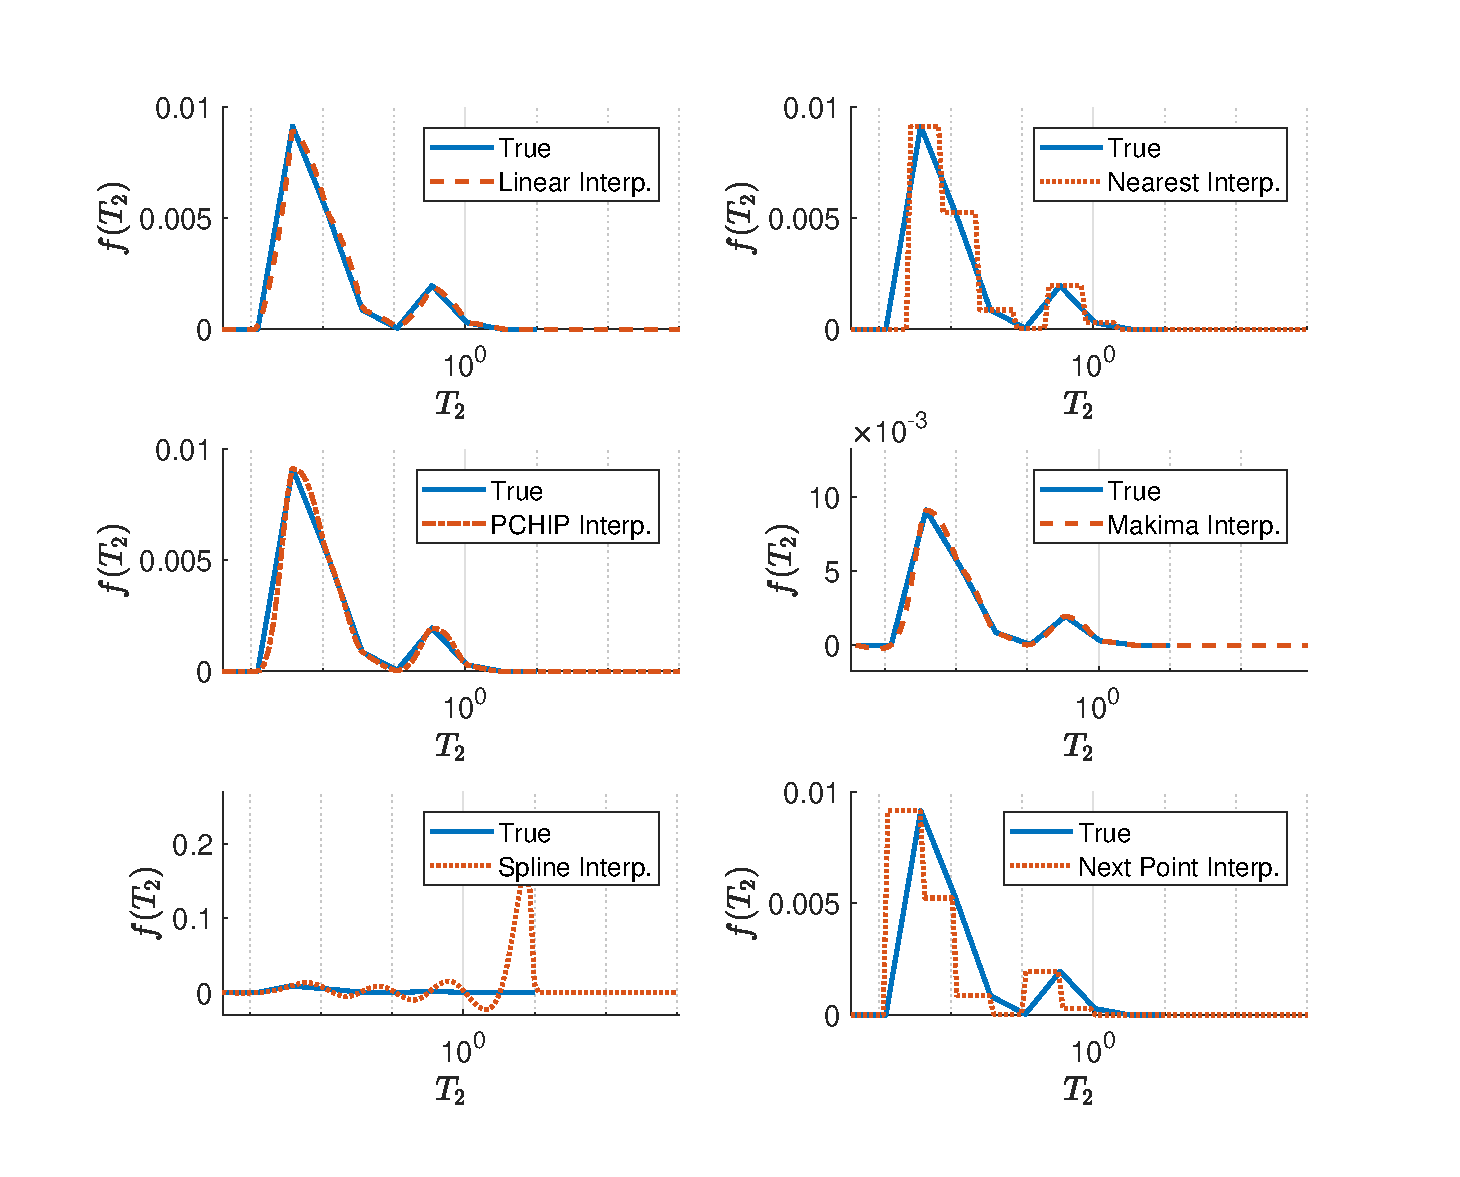
\includegraphics[width=\textwidth]{design/interpolation_choice.eps}
    \caption{Test of different interpolation techniques for interpolation from a lower dimensionality ($N_y = 10$) to a higher dimensionality ($N_y = 100$)}
    \label{fig:interpolation_comparison}
\end{figure}

Figure \ref{fig:interpolation_comparison} demonstrates different interpolation schemes for a conversion from 10 T2 relaxation bins to 100 T2 relaxation bins. Examining all of the candidate interpolation techniques, we can see the following:

\begin{enumerate}
    \item Nearest point and next point interpolation maintains the discretised coarseness of the original input function, making them poor at providing a representative T2 density function.
    \item The linear interpolation is less coarse than the nearest and next point interpolation techniques but it does not provide a smooth function. This makes it insufficient for providing a function with the expected smoothness of a density function.
    \item The spline interpolation \cite{cubicInterpolationMethods} and Makima (Modified Akima cubic Hermite) interpolation techniques \cite{akimaInterpolation} directly violate the non-negativity constraint on the density function.
    \item This leaves the shape-preserving piece-wise cubic interpolation (PCHIP) technique \cite{fritsch1980monotone} as the best candidate. It returns a valid non-negative function that is smooth. These two crucial aspects make it representative of a T2 density function attained through NMR relaxation.
\end{enumerate}

The resulting design decision made was to use PCHIP interpolation. It is fit-for-purpose in adapting experimental data to the Bayesian framework while preserving properties that accurately describe T2 relaxation.

\subsection{Estimation of the Prior Mean $\mu_f$}
\label{section:estPriorMean}
Computation of the mean of the prior involves taking the arithmetic mean of all of the experimental density functions over each of the T2 relaxation bins \cite{DiscreteRandomSignalsBookCovarianceEst}:

\begin{equation}
    \label{eq:mean_estimation_prior}
    \mu_f = \frac{1}{N_\text{rocks}} \sum^{N_\text{rocks}}_{i=1} f_i \quad \text{, where} \quad \mu_f \in \mathbb{R}^{N_{y}}
\end{equation}

 This is the estimation of the expectation of all of the T2 density functions of porous media that make up the experimental data.

\subsection{Estimation of the Covariance $C_f$}
The design choice of choosing the covariance estimator of the prior density function is concerned with balancing between measurement data and the prior information. Furthermore, there may be a dependence between each of the T2 relaxation bins that may be exploited to allow for a more robust estimator. 
Here we will analyse three candidate estimates for the covariance. These are that the prior covariance, $C_f$, is either:
\begin{enumerate}
    \item uniform and independent,
    \item non-uniform and independent, or
    \item non-uniform and dependent.
\end{enumerate}


\subsubsection{Method A -- Uniform Independent Covariance Estimation}\label{section:uniformIndependentCovar}
The first candidate of the estimation of the covariance assumes that the uncertainty for each T2 relaxation bin is uniform and independent. This makes the covariance equivalent to a scalar multiplied by an identity matrix:

\begin{equation}
    \label{eq:uniform_diagonal_covar}
    C_f = \sigma_\epsilon \cdot I
\end{equation}

This has the benefit of high generality as we can set a blanket uncertainty for our prior measurements. However, this also reduces the descriptiveness of the prior.

\subsubsection{Method B -- Non-Uniform Independent Covariance Estimation}
This estimation of the covariance of the prior density function takes into account the varying uncertainty for different T2 relaxation bins.
\begin{equation}
    \label{eq:nonuniform_diagonal_covar}
    C_f =      
    \begin{bmatrix}
    \sigma_{f_1}  \\
    \sigma_{f_2} \\
    \vdots \\
    \sigma_{f_{N_2}}
    \end{bmatrix} ^ T
    \cdot  I
    \text{,  where }
    \quad
    \sigma_{f_i} = 
    \sqrt{
    \frac{1}{N_{\text{rocks}}-1}
    \sum ^{N_{\text{rocks}}}_{j = 1}
    (f_{i,j} - \mu_i)^2
    }
\end{equation}

The assumption of independence leads to a covariance that is a positive definite diagonal matrix (all of the non-zero values are positive and on the diagonal). Though more flexible than method A, this assumes that the high quality experimental T2 relaxation bins do not have dependence on one another.



\subsubsection{Method C -- Non-Uniform Dependent Covariance Estimation}
This estimates the covariance directly from the high quality density functions \cite{DiscreteRandomSignalsBookCovarianceEst}.

\begin{equation}
    \label{eq:nonuniform_dependent_covar}
    C_f = \frac{1}{N_\text{rocks}} \sum^{N_\text{rocks}}_{i = 1} (f_i - \mu_f) (f_i - \mu_f)^T
\end{equation}


This models the dependence between different T2 relaxation bins in the density function. Hence, this covariance estimate fully describes the uncertainty and dependence of different points of the prior. However, it is more vulnerable to overfitting directly to the prior data we are using.



\subsubsection{Choosing the Covariance Estimate}
To make our choice of the covariance of the prior, we must determine which one tends to perform the best. The methodology of the experiment is as follows:
\begin{enumerate}
    \item Scale the covariance with a scalar, $\alpha$, such that we may see how the candidate over estimates and underestimates the true uncertainty. This is analogous to the regularisation in the approximate ILT in Section \ref{section:ILT}.
    \item Utilise leave-one-out cross validation (detailed in Section \ref{section:crossValidation}) so that the true density function we are estimating is unavailable to the estimator itself. This is so we may penalise overly specialised prior distributions. We average out all of the results with root mean square error so we may penalise estimation bias and variance equally \cite{StatisticsTextbookMSE}.
    \item Create an estimate of the BFV from the density function estimated by the posterior expression in (\ref{eq:posteriorProbability}) and compare with the true BFV. We operate at $T_c = 33$ ms as this will be the typical operating point for the estimator \cite{porousMediaT2Relaxation}. The BFV prediction uses the sharp integral transform (\ref{eq:sharpBFVIntegral}) given in Section \ref{sec:integralTransform}.
\end{enumerate}

\begin{figure}[tb!]
    \centering
    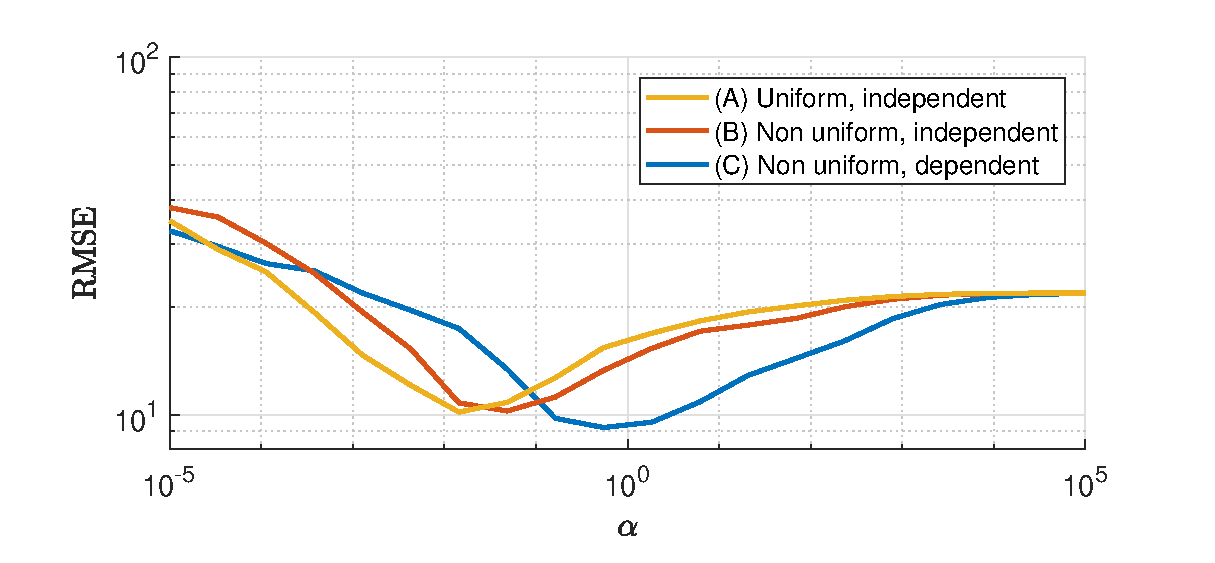
\includegraphics[width = 0.8\textwidth]{design/compare_covariance.eps}
    \caption{Comparison of the root mean square error of the estimator for the uniformly scaled candidate covariance estimates, $\alpha C_f$}
    \label{fig:RMSE_covariances}
\end{figure}

Figure \ref{fig:RMSE_covariances} illustrates the performance of the candidate estimates of the covariance at an SNR of 10. We see that the non-uniform and dependent covariance estimate (Method C) outperforms the other estimates for where $\alpha > 0.1$. Methods A and B at their best respective $\alpha$ are outperformed by method C. As we are looking for the best possible covariance prior, the non-uniform dependent covariance (Method C) is the most ideal. In the final design we utilise $\alpha = 1$ as it still outperforms the other estimates while simplifying the model with little cost.




\section{Integral Transform} \label{sec:integralTransform}
The goal of the estimator is to estimate the bound fluid fraction of a porous media sample, not the density function. Obtaining this value requires the computation of integral transforms of the estimated density function for the bound fluid volume and the porosity. The two types of BFV transforms are shown in Figure \ref{fig:bfv_integral_trans} for where $T_c = 33$ ms. Both candidate transforms are analysed in the comparative evaluation in Chapter \ref{C:evaluation}.

\begin{figure} [htb!]
    \centering
    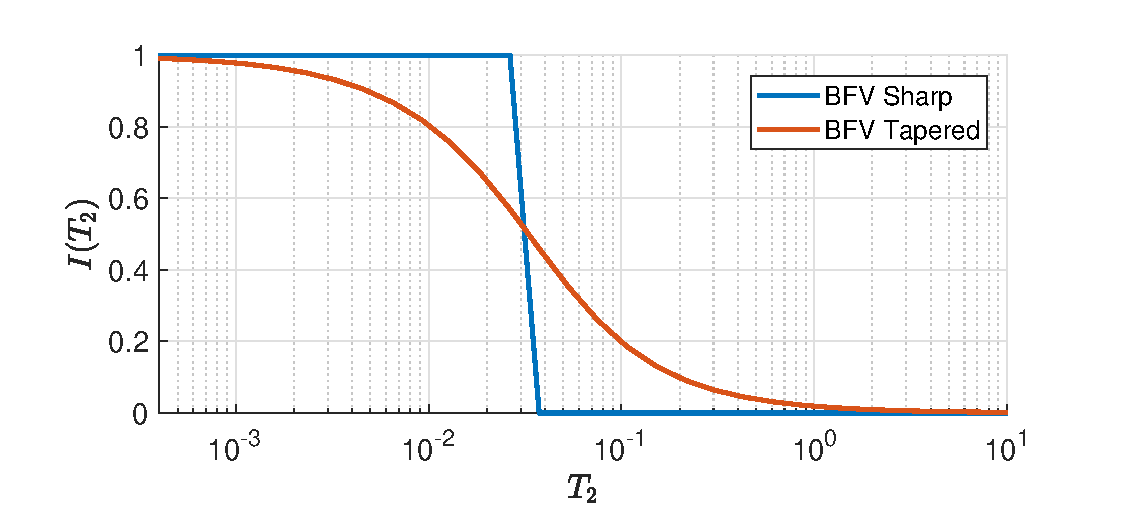
\includegraphics[width=0.8\textwidth]{design/bfv_integral.eps}
    \caption{Comparison of the BFV integral transforms for a bound fluid cut-off of $T_c = 33$ms}
    \label{fig:bfv_integral_trans}
\end{figure}

\subsection{Sharp Bound Fluid Volume}
The bound fluid volume is defined as the integration of the density function from $T_2=0$ to $T_2=T_c$ (\ref{eq:boundFluidVolume}). In the discretised version, this is equivalent to the inner product of the density function with a vector composed of ones for values below Tc and zeros for values above. There is no smooth transition from the bound fluid to the free fluid; hence, it is referred to as the sharp Bayes method. This is expressed as:

\begin{equation}
    \label{eq:sharpBFVIntegral}
    BFV_{\text{sharp}} = \int^{T_c}_{0} f(T_2) d T_2 \approx \text{step}(T_2 - T_c)^T f
\end{equation}

The strength of using an integral transform like this is that it is explicit with what it considers bound fluid volume. The weakness of this however is that it does not have any tolerance for `leaking' from one T2 relaxation bin to another. This is something that a noisy measurement can inflict onto an estimation of the density function. This brings into the picture another candidate; the tapered integral transform.


\subsection{Tapered Bound Fluid Volume}
Tapered integral transforms have a looser tolerance between bound and free fluid volume. A looser tolerance allows for a more robust estimator for noisy environments that may cause `leakage' between T2 relaxation bins. The candidate integral transform for comparison with its sharp counterpart is the exponential Haar transform (EHT) proposed by Gruber et al. \cite{GruberLinearFunctionals2013}. The discretised version or this is the inner product between a discretised EHT and the density function. This is depicted analytically as:

\begin{equation}
    \label{eq:taperedBFVIntegral}
    BFV_{\text{tapered}} = \int^{\infty}_{0} K_{\text{EHT}}(T_2,T_c) f(T_2) dT_2 \approx  K_{\text{EHT}}^T f
\end{equation}


\subsection{Porosity}
Calculating the porosity of the discretised density function is more straightforward. It is by definition the sum of all the T2 relaxation bins (\ref{eq:porosity_defn}). This is an approximation of the integration of the density function over the entire T2 domain.

\section{Metrics}
A vital aspect of estimation is to have defined metrics to evaluate and compare different techniques. The goal in this part of the design is to fairly evaluate the viability and effectiveness of the different techniques in a balanced manner.


\subsection{Error}
The error of the estimated BFF will take the form of an absolute error. A comparative error is used instead of comparing the actual BFF estimate as we are utilising cross validation over thirty different samples of high quality experimental data. We want to establish a generalised measure of performance.

To visualise the spread and bias, we will use the empirical cumulative distribution functions (CDFs). These are especially advantageous as we may directly compare the cumulative probability of the error for different techniques. We may explicitly state the likelihood of a degree of error so that we may see how performance varies for different magnitudes of acceptable error.

\subsection{Computational Effort}
Though not exhaustive, the computation time of the algorithm reveals a useful comparative perspective on feasibility. For an algorithm to be feasible in the field, it should have a similar or lower computation time to other techniques. The computer and its computational load are held constant. Several repeated results are taken to obtain a general distribution of the computation time.


\section{Design Conclusions}
The consideration of the several intricacies of the Bayesian framework has made its development possible. The flexibility of a Gaussian density prior combined with the analytic expression in (\ref{eq:bayes_multivariate_dist}) provides a strong case for its implementation. The following chapter explores the implementation of this design so that it may be compared with other techniques in the literature.





\chapter{Implementation}\label{C:implementation}
The Bayesian estimator proposed in this report has required comprehensive technical implementation to provide a strong comparative analysis of its effectiveness. These components include:

\begin{itemize}
    \item implementation of techniques proposed by previous studies for this problem domain,
    \item the validation of the implementation of those competing techniques such that each of their distinct features can be accurately compared and analysed,
    \item creation of the proposed estimator with consideration for its special input requirements compared to the previous techniques, and
    \item a fair test procedure and algorithm to compare and contrast the different estimators.
\end{itemize}

These several components were developed, prototyped, and analysed in \textit{MATLAB}. This is such that the analysis may be general. Therefore, the results from here can be transferred towards other platforms such as an embedded implementation.



\section{Existing Techniques}
The existing techniques were implemented and validated against the published results. This allows for analysis beyond the specific case study density functions discussed within their respective publications. This means that we may obtain a valid comparison of methods via a larger variety of representative data. In addition, there is no known publicly published implementation of the techniques by the authors, hindering implementation.

\subsection{Validation of Implementation}
The validation framework compares an extraction of the original estimate with the reproduced estimate. This allows for an accurate perspective of any analysis made between the benchmark estimators and the proposed estimator. Figure \ref{fig:validate_recreated_models} demonstrates the validation topology used by this project.

\begin{figure}[h]
    \centering
    \includegraphics[width=\textwidth]{implementation/ValidateRecreatedModels.pdf}
    \caption{Test architecture for recreating the existing estimators in the literature}
    \label{fig:validate_recreated_models}
\end{figure}

The components of the validation framework process are as follows:

\begin{enumerate}
    \item The image extractor uses an image of the model in the publication to acquire the published density function and its technique's estimate. An off the shelf image extractor was used \cite{webplotdigitizer}.
    \item The interpolator discussed in Section \ref{section:oneDimInterpolation} is used so we may have direct compatibility and comparability between the different frameworks
    \item The estimator being validated develops its estimate of the density function
    \item The comparison component allows for analysis of the deviations between the true estimate and the recreated estimate. This takes the form of visual display and the numerical indicators of error and deviation.
\end{enumerate}

We use the published model density functions analysed by Gruber et al. \cite{GruberT2Estimation2013} for the validation of the different recreations of the techniques. This means that any analysis we make on technique accuracy here may be representative of actual data. Figure \ref{fig:T2_validation_models} illustrates each of the models used for system validation.

\begin{figure}[htb!]
    \centering
    \begin{subfigure}[b]{0.49\textwidth}
        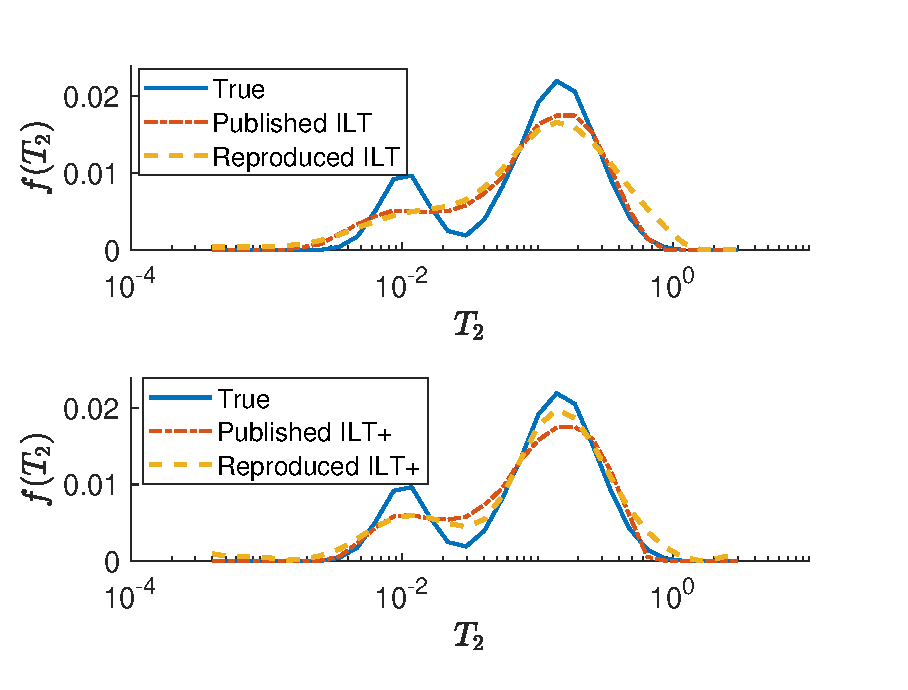
\includegraphics[width=\textwidth]{implementation/model1.eps}
        \subcaption{Model \#1}
        \label{fig:model1True}
    \end{subfigure}
    \begin{subfigure}[b]{0.49\textwidth}
        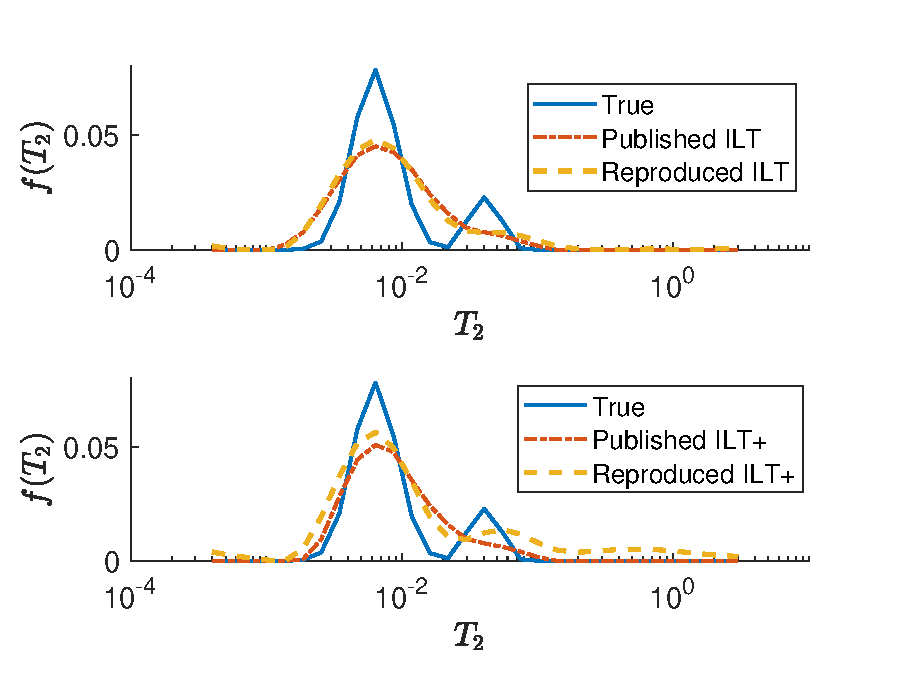
\includegraphics[width=\textwidth]{implementation/model2.eps}
        \subcaption{Model \#2}
        \label{fig:model2True}
    \end{subfigure}
    \begin{subfigure}[b]{0.49\textwidth}
        \includegraphics[width=\textwidth]{implementation/model3.eps}
        \subcaption{Model \#3}
        \label{fig:model3True}
    \end{subfigure}
    \begin{subfigure}[b]{0.49\textwidth}
        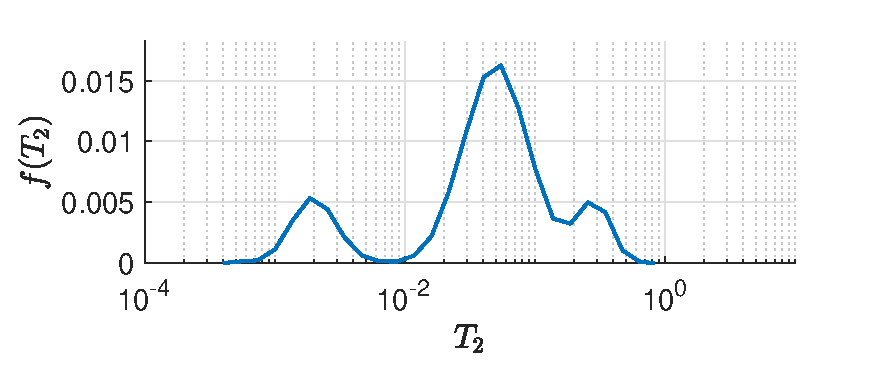
\includegraphics[width=\textwidth]{implementation/model4.eps}
        \subcaption{Model \#4}
        \label{fig:model4True}
    \end{subfigure}    
    \caption{The $T_2$ density functions of the models used for system validation}
    \label{fig:T2_validation_models}
\end{figure}


\subsection{Inverse Laplace Transform Approximation (ILT)} \label{section:ILTImplementation}
The canonical benchmark for density function estimation is the ILT approximation detailed in \cite{Venk2DFredholm2002} and Section \ref{section:ILT}. This project explores one-dimensional density functions rather than the two dimensional kind detailed by Venkataramanan et al. \cite{Venk2DFredholm2002}. This meant that the re-implementation tended towards the one-dimensional case proposed by the Butler-Reeds-Dawson method instead \cite{BulterReedsDawsonMethod1981}.




\subsubsection{Non-uniform SNR}
The simulation implementation from Gruber et al. \cite{GruberT2Estimation2013} is complicated by the inclusion of additional short pulse sequences that accompany the typical long pulse sequence. There are a series of thirty pulses repeated 10 times that increase the SNR for short relaxation times. This means that to reproduce the technique exactly, this component had to be reproduced as well. The method of implementation is as follows:

\begin{enumerate}
    \item Simulate the data for only 30 samples in the time domain 10 times (short pulses)
    \item Average these 10 pulse sequence results together
    \item Replace the first 30 values of the long sequence with the new averaged short pulse sequence results
    \item Scale the first 30 rows of the kernel matrix, $K$, by the SNR increase given by the short pulse sequence. We do the same for the measurement vector.
\end{enumerate}

\begin{figure}
    \centering
    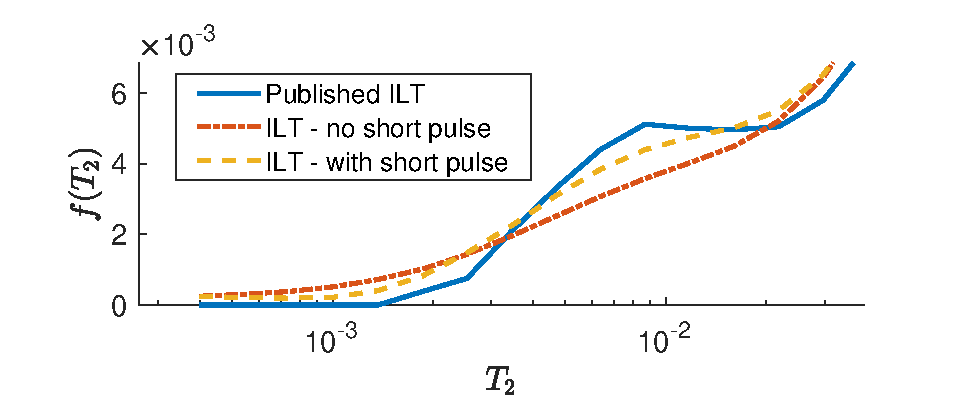
\includegraphics[width = 0.9\textwidth]{implementation/recreate_short_pulse.eps}
    \caption{Recreation of model 1 (Fig. \ref{fig:model1True}) ILT from Gruber et al. \cite{GruberT2Estimation2013} with and without the inclusion of repeated short pulse sequences.}
    \label{fig:non_uniform_SNR}
\end{figure}
 Figure \ref{fig:non_uniform_SNR} demonstrates the effect of accounting for a short pulse sequence in estimator recreation. As we can see, the reproduced technique's estimate is more sensitive for short relaxation. This in turn corresponds to a closer reproduction to the published result. Therefore, this methodology provides a more accurate representation of short relaxation times for our reproduction of the ILT experimental results in \cite{GruberT2Estimation2013}.




\subsubsection{Scaling the Noise}
The published noise standard deviation of 0.1 and an SNR of 10  in \cite{GruberT2Estimation2013} requires that the signal power be unity. However, the density functions benchmarked in the publication do not have unity power, i.e, the power of the measured signal before noise is added is not unity ($P_{\text{signal}} = \frac{1}{N_2}\sum^{N_2}_1 (m_i)^2 \neq 1$). Therefore, the noise standard deviation is scaled to achieve the published SNR such that the results can be recreated.

\subsubsection{$T_2$ Axis}
The $T_2$ axis of the density function estimate is a crucial aspect to reproduce due to the high variability that may come from an ill-conditioned problem.
The time axis was assumed to be defined for times from $2\times t_\text{sample}$ to 3 seconds as the simulation results in \cite{GruberT2Estimation2013} are bounded within these values. The $2\times t_\text{sample}$ bound is justified by the Shannon Sampling theorem \cite{shannon1949communication}. A sample period of $t_\text{sample}$ may only fully reconstruct T2 relaxation times of more than $2\times t_\text{sample}$ . In addition, the attention to this specific aspect of an inversion is justified by recent research into estimation sensitivity for that region of the $T_2$ domain \cite{venkataramanan2015newPorosity}.

\subsection{ILT+}
This technique requires a significant amount of complexity as it combines moment estimation by Venkataramanan et al. \cite{VenkMellin2010}, tapered area estimation by Gruber et al. \cite{GruberLinearFunctionals2013}, and the initial ILT methods by Venkataramanan et al. \cite{Venk2DFredholm2002} and Butler et al \cite{BulterReedsDawsonMethod1981}. The implementation follows many of the same points as the ILT method discussed in Section \ref{section:ILTImplementation}.

\begin{figure}[ht!]
    \centering
    \begin{subfigure}{1\textwidth}
        \centering
        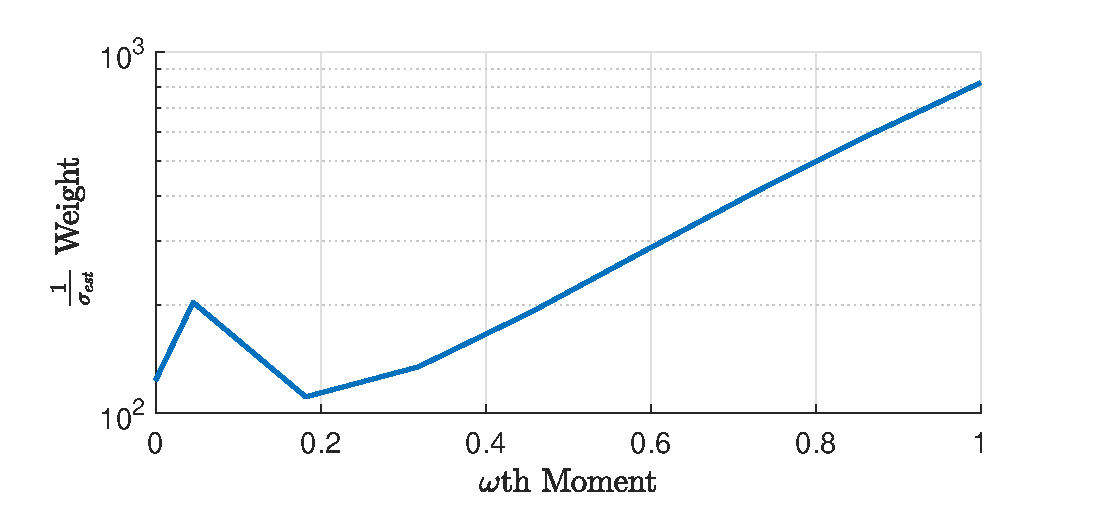
\includegraphics[width=0.8\textwidth]{implementation/moment_weighting.eps}
        \subcaption{Weighting of each moment estimation's certainty on a logarithmic scale}
    \label{fig:moment_estimator_weight}
    \end{subfigure}
    \begin{subfigure}{1\textwidth}
        \centering
        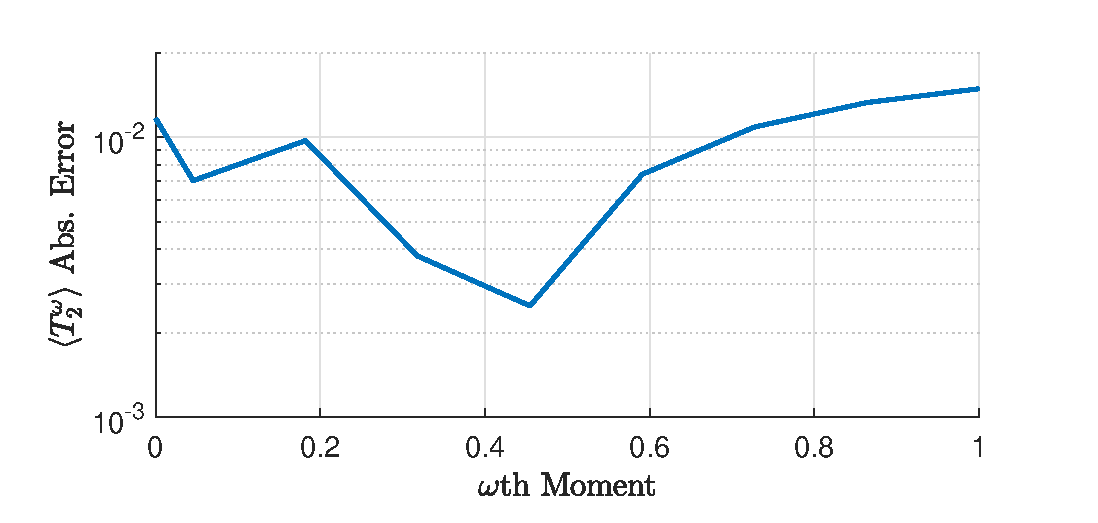
\includegraphics[width=0.8\textwidth]{implementation/moment_abs_error.eps}
        \subcaption{Absolute error of the moment estimation on a logarithmic scale}
        \label{fig:moment_estimator_abs_err}
    \end{subfigure}
    \caption{A comparison of the certainty alongside the absolute error of the reproduced moment estimate for SNR = 10.}
    \label{fig:problems_moment_est}
\end{figure}

\subsubsection{Moment Estimator} \label{section:moment_est_implementation}
The ILT+ implementation was adversely complicated by the inclusion of the moment estimator detailed in Section \ref{section:moment_estimation} and given by Venkataramanan et al \cite{VenkMellin2010}. One of the main problems with it was with robustness and error. In order to compensate for this, we modify its weighting so that we may at least acquire indicative results for the evaluation in Chapter \ref{C:evaluation}.




To demonstrate a problem encountered in implementing the moment estimator in the estimator framework, we examine the moment estimation for model 1 from Gruber et al \cite{GruberT2Estimation2013} (shown in Figure \ref{fig:model1True}). 



Figure \ref{fig:moment_estimator_weight} indicates that as higher moments are estimated, we have a higher weighting for that estimate. However, in Figure \ref{fig:moment_estimator_abs_err} we can see that the absolute error increases for where $\omega > 0.5$. This is problematic as the implementation weights these more erroneous points more highly, i.e. the optimisation framework is more certain about worse estimates.

Given this issue with the implemented moment estimator there is a need to diminish its dependence on worse estimates. This diverges from the published results. However, we still preserve indicative trends of performance for the comparative analysis.

\begin{figure}[htb!]
    \centering
    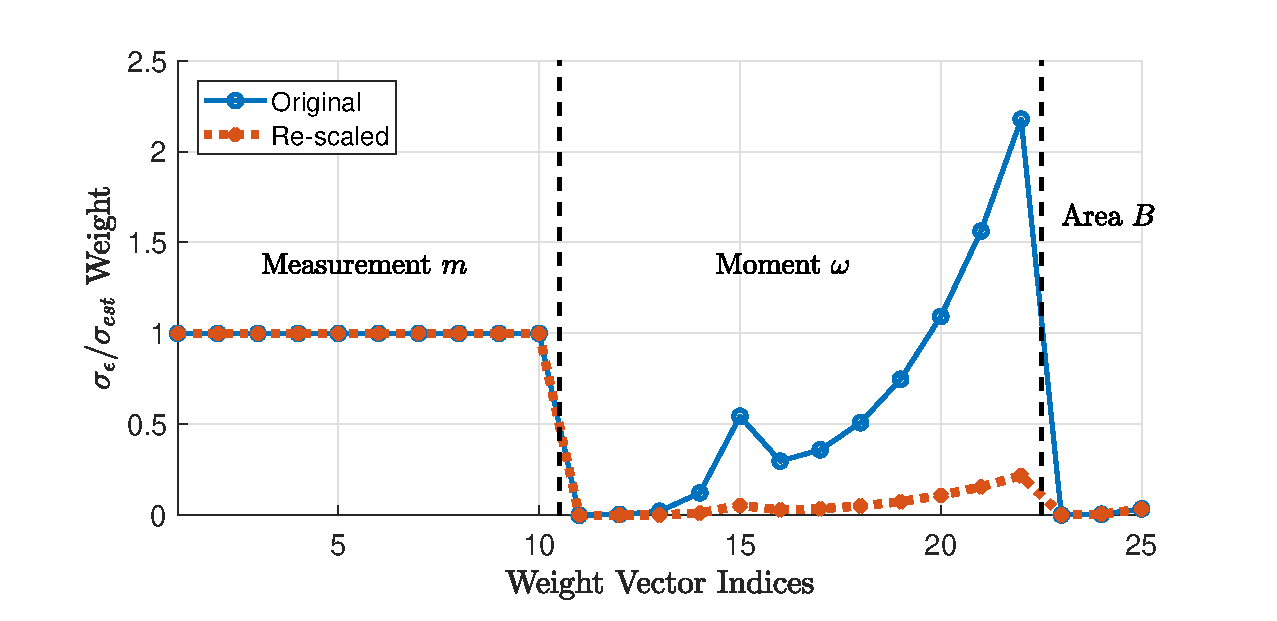
\includegraphics[width = 0.9\textwidth]{implementation/new_weighting_iltx.eps}
    \caption{Comparison of the original and altered weight vectors for ILT+ to allow for analysis of general indicative performance}
    \label{fig:diff_ILT+}
\end{figure}

Figure \ref{fig:diff_ILT+} demonstrates the augmented weighting regime for our implementation of ILT+. The moment weightings are reduced tenfold while all others remain the same so that the moment estimation may not overpower the overall estimation. This amount of reduction was done so that the implementation of the ILT+ would follow to an extent the published ILT+ results.





\iffalse
\subsubsection{Regularisation for ILT+}
The starting regularisation value used before the iterative process has a large effect on the resulting estimate for the ILT+ using the BRD method \cite{BulterReedsDawsonMethod1981}. For example, if the initial $\alpha$ were a very low number such as 0.1 to 1 (less than 10\% the published regularisation average), the result would require inversion of a poorly conditioned matrix. A large $\alpha$ on the other hand has a more stable start point. Figure \ref{fig:ilt+sensitivity} demonstrates the difference in an ILT+ estimate from choosing a different regularisation parameter with the same random seed. This aspect severely impacts implementation and make it difficult to reproduce the published results.

\begin{figure}
    \centering
    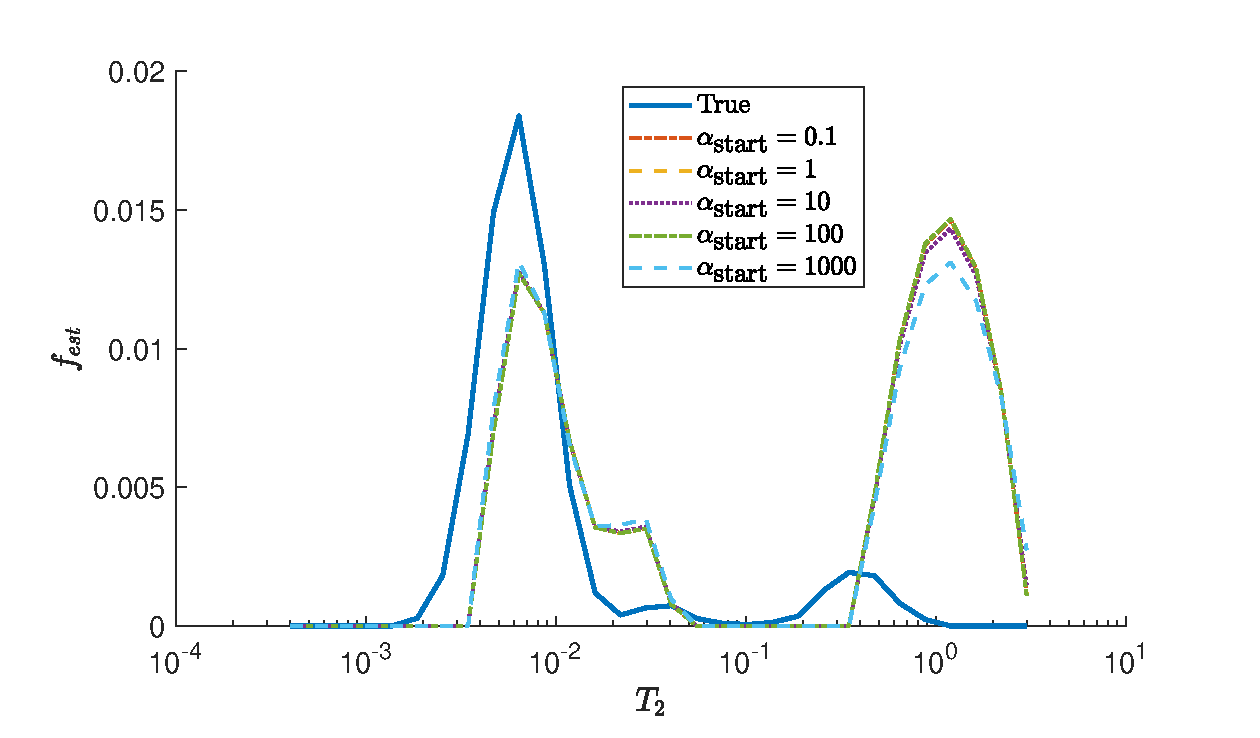
\includegraphics[width=\textwidth]{implementation/ILT+Regularisation.eps}
    \caption{Sensitivity to a start $\alpha$ in inversion for ILT+}
    \label{fig:ilt+sensitivity}
\end{figure}
\fi

\subsection{Tapered Area Estimator}
The tapered area estimator has a far simpler set up compared to the previous approximation techniques. This is due to it being fully self-contained and analytically tractable. It contains the exponential Haar transform detailed in \cite{GruberLinearFunctionals2013} and Section \ref{ss:taperedAreas}. It is a simple dot product between the time domain version of the transform and the measurement data per (\ref{eq:estTaperedAreas})

\section{Bayesian Technique}
The implementation of the Bayesian technique is more comparable to the tapered area estimator rather than the regularised least squares methods of the ILT and ILT+. This is due to the Gaussian assumption of the prior density function and the measurement data permitting an analytic approach to implement the estimator (as discussed in Section \ref{section:bayesTechniqueDesign}). The implementation is compared with the results obtained by Teal to allow for validation \cite{paulTeal_NMRBayes}.

\subsection{Estimator Architecture}
We adopt a computational sequence for the Bayesian technique to minimise unnecessary computation. The sequence, as shown also in Figure \ref{fig:bayesian_framework}, is as follows:
\begin{enumerate}
    \item we take the high quality known density functions and construct our prior mean and covariance before any time sensitive procedures. The prior can be constructed before estimation
    \item calculate the estimate density function, the mean of the Bayesian posterior, using (\ref{eq:posteriorProbability})
\end{enumerate}


The procedure requires no iterative computation like the ILT and ILT+, providing potential for less computation time. This is because the time consuming computation of the prior function does not have to be done within time-constrained use.






\section{Test Environment}
The test environment's implementation required attention so that it provided immediate comparability and fairness. The implementation of the test environment is required to be such that it provides an illuminating and fair comparison of the different techniques. The code for this can be found in \cite{dobbie_2018_test_Env}.


\subsection{Test Architecture}
The test architecture that compares each of estimators aims to demonstrate the uncertainty and typical performance of all of the techniques. In order to keep the Bayesian estimator from directly accessing the exact sample it is testing, leave one-out cross validation (as discussed in Section \ref{section:crossValidation}) is utilised for the evaluation process. Figure \ref{fig:test_architecture} details the architecture of the test setup. Table \ref{tab:test_variables} outlines the variables set for this test architecture. Any variation from these variables in the evaluation will be explicitly stated.


\begin{table}[h]
    \centering
    \begin{tabular}{l c l}
        \toprule
         & Variable  &     \hfill   Experimental Value \\
        \midrule
        $N_2$ & Number of Time Samples & 2500 \\
        $N_y$ & Number of Bins in T2 domain & 30 \\
        $t_E$ & Sample Period & \SI{200}{\micro\second}\\
        $T_2$ & Axis Bounds & \SI{400}{\micro\second} to 10 s \\
        $SNR_{\text{linear}}$ & Signal to Noise Ratio (Uniform) & 10 \\
        $T_c$ & Bound Fluid Cut-off & 33 ms \\
        \bottomrule
    \end{tabular}
    \caption{The variables used for the test architecture.}
    \label{tab:test_variables}
\end{table}



\begin{figure}[h]
    \centering
    \includegraphics[width=\textwidth]{implementation/test_arch2.pdf}
    \caption{The overall test setup to compare each of the estimators fairly.}
    \label{fig:test_architecture}
\end{figure}



An extension of the test architecture can allow for an analysis of how different cut-off times lead to different performance. This provides a perspective of when one technique may be more suitable than another technique. This comes at the cost of computational time, as estimating many samples over $N_y$ different cut off times for several techniques requires a non-trivial amount of computation. 


\subsection{Implementation Conclusions}

Throughout Chapter \ref{C:implementation}, there has been detailed analysis of the implementation of each of the estimators. Most of the complications came from quality issues in reproducing the existing techniques. The absence of published code by the authors made high quality reproduction non-trivial. However, the compromises made still allow for an indication of typical technique performance and trends. These aspects allow for the detailed evaluation in Chapter \ref{C:evaluation}.






\iffalse
In addition to the test environment, there is also a visual comparison of different case study density functions. There are published results by Gruber et al. \cite{GruberLinearFunctionals2013} that form a typical benchmark of the density functions that will be estimated. Even though some of the previously published results could not be reproduced exactly in the re-implemented estimators, the Bayesian technique can still be compared with definitive previous results.
\fi
\chapter{Evaluation}\label{C:evaluation}
Due to the variable nature of statistical estimation, there are several different perspectives that will be explored. Primarily, the Bayesian technique will be compared and benchmarked with the literature's competing methods. This will be analysed in terms of error between the technique's estimate BFF and the true BFF of the sample.

We evaluate the estimators via different perspectives of usability, such as : 
\begin{itemize}
    \item accuracy at the typical $T_c$ for sandstone rock and at a typical expected SNR environment given by \cite{GruberT2Estimation2013}, the target operating point of the estimator, 
    \item robustness of the estimation with respect to predicting different bound fluid cut off times, 
    \item sensitivity towards different SNR environments such that we may consider application for different noise powers, 
    \item robustness of the Bayesian estimator to different sample sizes making up the prior, and
    \item computation speed to indicate potential compatibility with different platforms.
\end{itemize}

\begin{figure}[htb!]
    \centering
    \begin{subfigure}[b]{0.49\textwidth}
        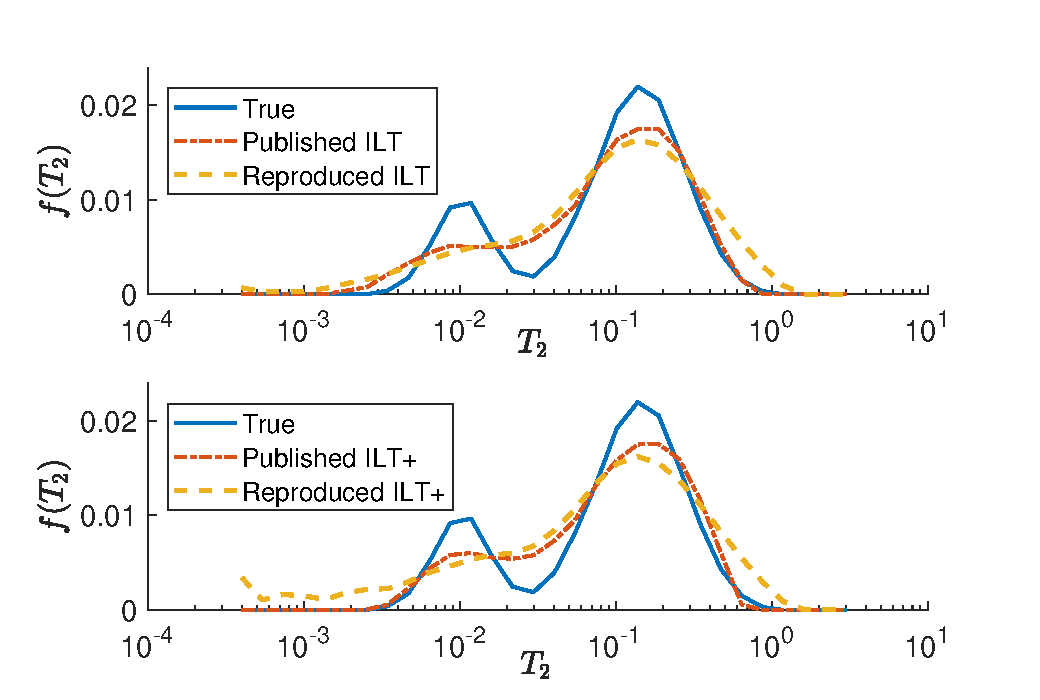
\includegraphics[width=\textwidth]{evaluation/model1_recreate.eps}
        \subcaption{Model \#1}
        \label{fig:model1Recreation}
    \end{subfigure}
    \begin{subfigure}[b]{0.49\textwidth}
        \includegraphics[width=\textwidth]{evaluation/model2_recreate.eps}
        \subcaption{Model \#2}
        \label{fig:model2Recreation}
    \end{subfigure}
    \begin{subfigure}[b]{0.49\textwidth}
        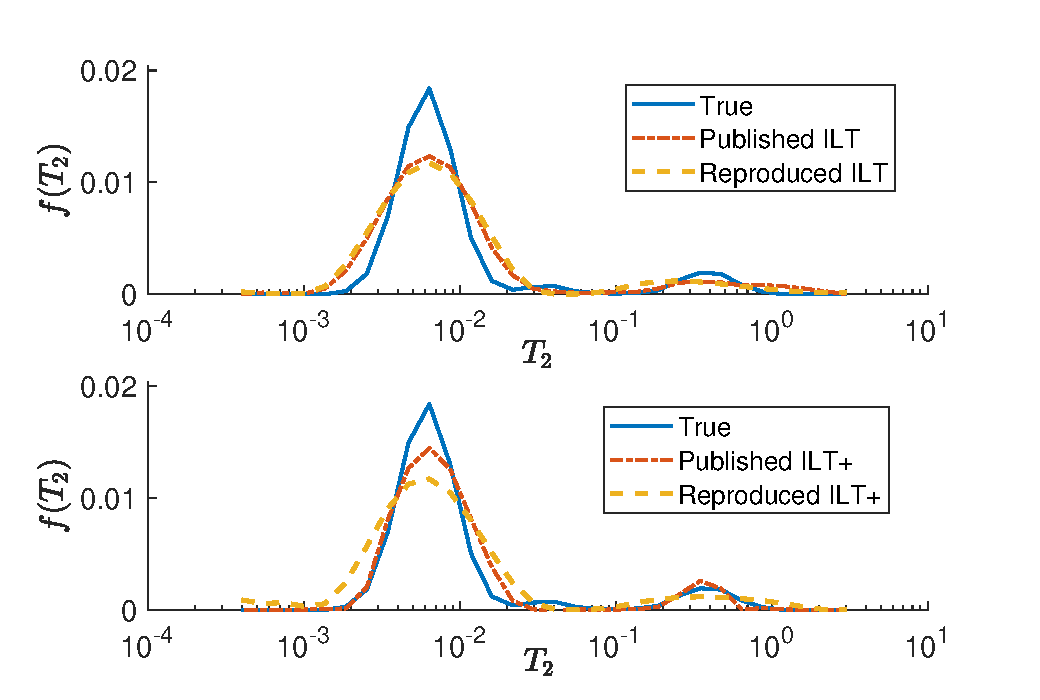
\includegraphics[width=\textwidth]{evaluation/model3_recreate.eps}
        \subcaption{Model \#3}
        \label{fig:model3Recreation}
    \end{subfigure}
    \begin{subfigure}[b]{0.49\textwidth}
        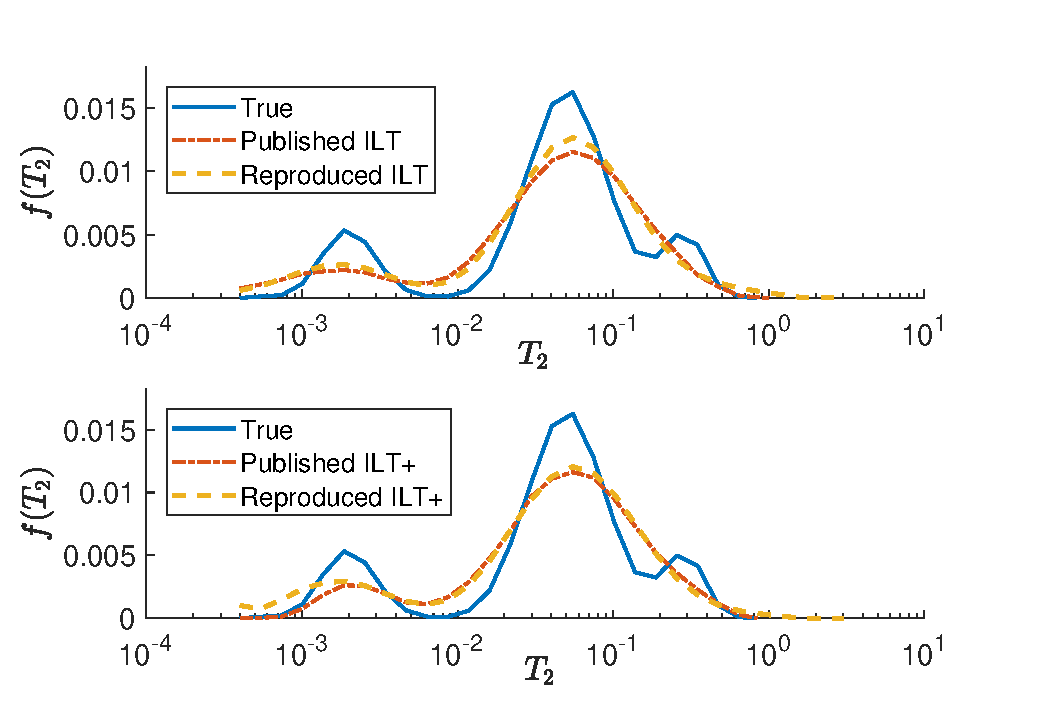
\includegraphics[width=\textwidth]{evaluation/model4_recreate.eps}
        \subcaption{Model \#4}
        \label{fig:model4Recreation}
    \end{subfigure}    
    \caption{The mean estimated $T_2$ distribution of the recreated of ILT and ILT+ methods}
    \label{fig:mean_recreated}
\end{figure}

\section{Recreated Algorithm's Closeness}
The analysis in this section utilises the same experimental conditions as detailed in \cite{GruberT2Estimation2013}. These results specifically compare algorithm recreation for an SNR of 10. The truncated singular value decomposition compression of the measurement data preserves the 10 largest singular values per \cite{GruberT2Estimation2013}.



The reproductions of the ILT and ILT+ techniques are compared with published results by Gruber et al \cite{GruberT2Estimation2013} in Figure \ref{fig:mean_recreated}. The ILT+ technique is particularly erroneous for relaxation times below 3 ms. This is likely to be an error in the implementation of the moment estimator as discussed in Section \ref{section:moment_est_implementation}. Nevertheless, the reproduced techniques, even with error in the replication of the ILT+, still provide some indication of the typical performance of these techniques.

Table \ref{tab:reproductionError} demonstrates the difference between the overall signal error in implementation and the signal power (porosity of the sample, $\phi$) of the overall estimate. We see that the error from estimation tends to be below 10\% for the typical density functions. This error does not overwhelm the estimated signal. This means that reproduced performance is indicative of the true application of the algorithm. In addition, if there is a performance gap beyond 10\% in the evaluation, it means the implementation error is unlikely to invalidate the performance comparisons made.


\begin{table}[htb!]
\centering
    \begin{tabular}{l p{1.75cm} p{1.75cm} p{1.75cm}  p{1.75cm} p{1.75cm} p{1.75cm}}
    \toprule
    	& Reprod. ILT Error $\phi_E$ & Published ILT $\phi$ & ILT Error $\frac{\phi_E}{\phi}$ & Reprod. ILT+ Error $\phi_E$ & Published ILT+ $\phi$ & ILT+ Error $\frac{\phi_E}{\phi}$  \\
    \midrule
	Model 1 & 1.13E-2 & 0.1502 & 7.52\% & 1.48E-2 & 0.1507 & 9.82\% \\ 
	Model 2 & 1.31E-2 & 0.2911 & 4.50\% & 2.3E-2 & 0.2854 & 8.06\% \\ 
	Model 3 & 9.4752E-4 & 7.3800E-2 & 1.28\% & 9.100E-3 & 6.94E-2 & 13.11\% \\
	Model 4 & 5.3E-3 & 0.1024 & 5.18\% & 7.00E-3 & 0.1013 & 6.91\% \\ 
    \bottomrule

    \end{tabular}
        \caption{Error for the mean of the reproduced ILT and ILT+ density function estimates compared to the published results' mean estimate in \cite{GruberT2Estimation2013}. The values published here are unit less in correspondence with published results.}
    \label{tab:reproductionError}
\end{table}








\section{Technique Comparison for a Chosen $T_c$} \label{section:aChosenTc_evaluation}
The analysis made here is for the typical bound fluid cutoff for sandstone: $T_c = 33$ ms \cite{UsingNMRPetrophysicalKenyon1992nuclear}. Figure \ref{fig:cdf_all_tech} illustrates an empirical cumulative distribution function (CDF) of the absolute error of the estimate bound fluid fraction. The closer the line is to the y axis, the more better it is for a given cumulative probability.

As we can see from Figure \ref{fig:cdf_all_tech}, the Bayesian estimator with the sharp BFV integral transform outperforms all of the other techniques except for at the 99\% probability point of the CDF. It has 80\% of all estimated $BFF$ below an absolute error of 0.062. Comparatively, the performance of the Bayesian estimator with the tapered BFV integral transform is close to that of the ILT method. 80\% of both the Bayesian tapered and ILT techniques have an absolute estimation error of up to 0.1200. This 50\% reduction of error at this cumulative probability indicates a strong case for the viability of the Bayesian framework.

As we move our analysis towards the 95\% probability threshold of error, the sharp BFV Bayes and ILT+ methods' performance gap becomes smaller. Specifically, the Bayes Sharp BFV has 95\% of all BFF estimations with an absolute error below 0.1295. The reproduced ILT+ in comparison has 95\% of its estimations below an absolute error of 0.1479. 

The EHT method appear to have undoubtedly the worst performance out of all of the compared techniques. This is likely due to it being the least comprehensive form of estimation. It involves only one integral transform while the other methods include optimisation or a comprehensive prior.

\begin{figure}[htb!]
    \centering
    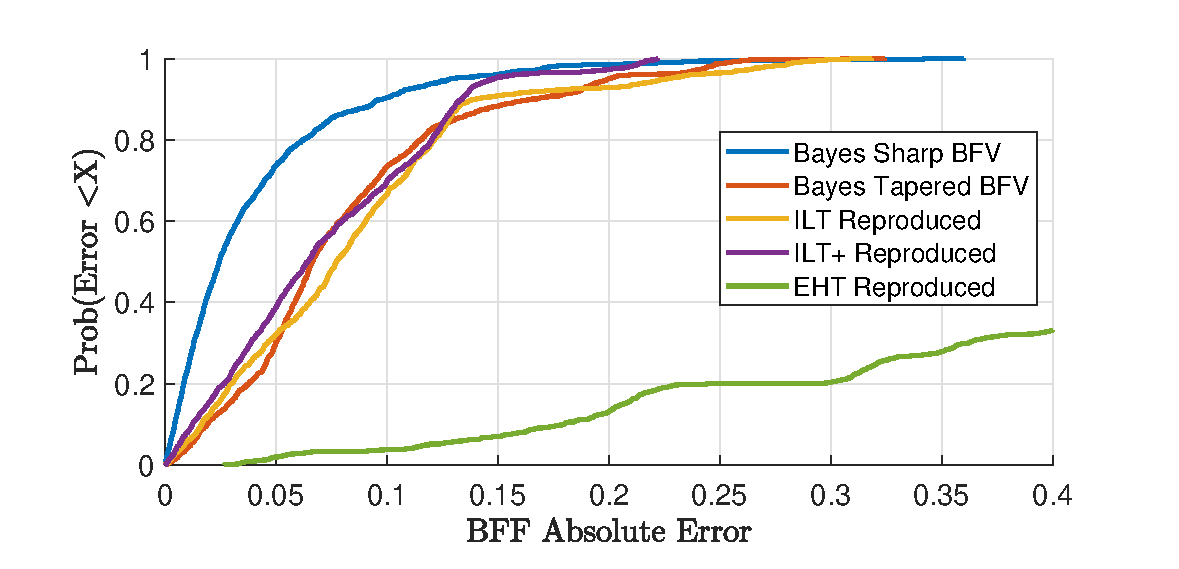
\includegraphics[width=\textwidth]{evaluation/main_analysis_plot.eps}
    \caption{Cumulative distribution function of the $BFF$ absolute error from the test architecture with respect to the experimental variables given in Table \ref{tab:test_variables}}
    \label{fig:cdf_all_tech}
\end{figure}

\section{Performance for Different $T_c$} \label{section:differentTc_evaluation}
When we expand the analysis towards a range of different cut-off times for bound fluid fraction, we notice the superior performance of the sharp BFV Bayesian estimator. Figure \ref{fig:TestDifferentTc} illustrates that the sharp BFV transform performs considerably better than the other techniques except for where $T_c$ lies between 1 ms and 6 ms. At the typical operating points of a bound fluid cut-off of 33 ms (for sandstone) and 90 ms (for carbonates) \cite{wellLoggingBook}, the sharp Bayes technique far outperforms the other techniques, by up to 0.025 in the estimation error. 

\begin{figure}[htb!]
    \centering
    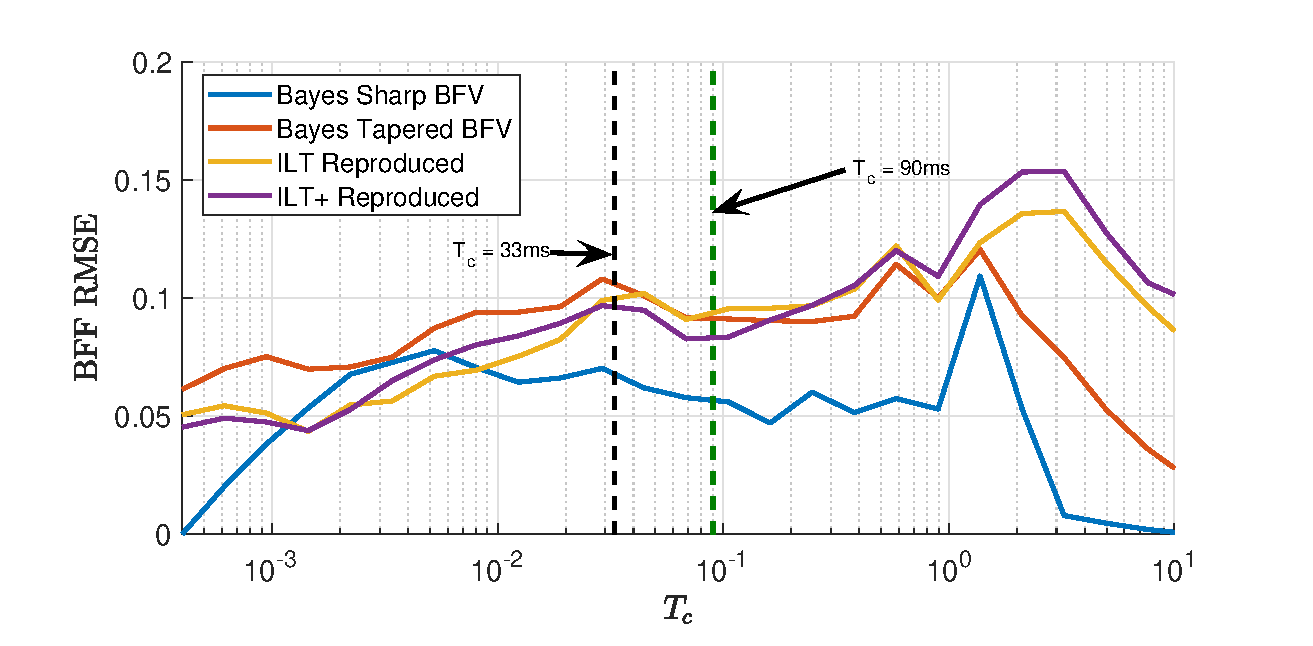
\includegraphics[width = \textwidth]{evaluation/different_Tc.eps}
    \caption{Root mean square error for different $T_c$, SNR = 10. The EHT has been omitted from this analysis to allow closer analysis of the more viable techniques}
    \label{fig:TestDifferentTc}
\end{figure}

The tapered Bayes technique in comparison performs poorly compared to the sharp Bayes technique. This implies that compensating for leaks between the T2 relaxation bins impairs performance. At no point does the tapered method outperform the sharp method. It performs closest to the sharp BFV technique in the short relaxation region of $T_c$ = 2 ms to 4 ms.

The sharp BFV Bayes estimator has an RMSE of less than 0.01 at the bounds of the T2 axis. This indicates that there is little leakage between the density function bins and hence the estimate BFF. This would be due to a near zero prior density function at these T2 relaxation times for all of the experimental density results. The other techniques have a degree of leakage between the relaxation bins that cause non-zero error in their cases. This is an operating region where the descriptive prior of the Bayesian estimator is at its most advantageous.




\section{Performance for Different $SNR$} \label{section:differentSNR_evaluation}
Estimation of the BFF will be typically done in environments with a potentially variable amount of noise power. This section of the evaluation explores how SNR affects estimation error. Figure \ref{fig:Comparative_SNR} illustrates an empirical CDF of absolute error for the techniques at different SNR values.  

We see that the sharp Bayes method  typically performs better than all of the other techniques for each of the different SNRs. For a lower SNR we observe that the sharp Bayes technique tends to perform more similarly to the ILT benchmark. The performance difference becomes more apparent at higher SNR.

As we examine the 80\% cumulative probability bound of the error, we see that that as the SNR increases, the sharp BFV Bayes estimator widens the performance gap between the competing techniques. For example, at a poor measurement SNR of 1 the error gap between the ILT and Bayes Sharp BFV is 0.0332. As the SNR increases to 100, this gap more than doubles to an error difference of 0.0766. 

We must note that as we examine performance at an increasingly high SNR, we begin to leave the scope the estimator aims to satisfy. This is because high quality experimental results are supposed to be tightly controlled and not influenced by prior information. Detailed prior information may only be suitable in noisier environments where we are unable to control much of the experiment. In those cases, we may accept the use of more detailed prior information to form an estimate. 


\begin{figure}[htb!]
    \centering
    \begin{subfigure}[b]{0.49\textwidth}
        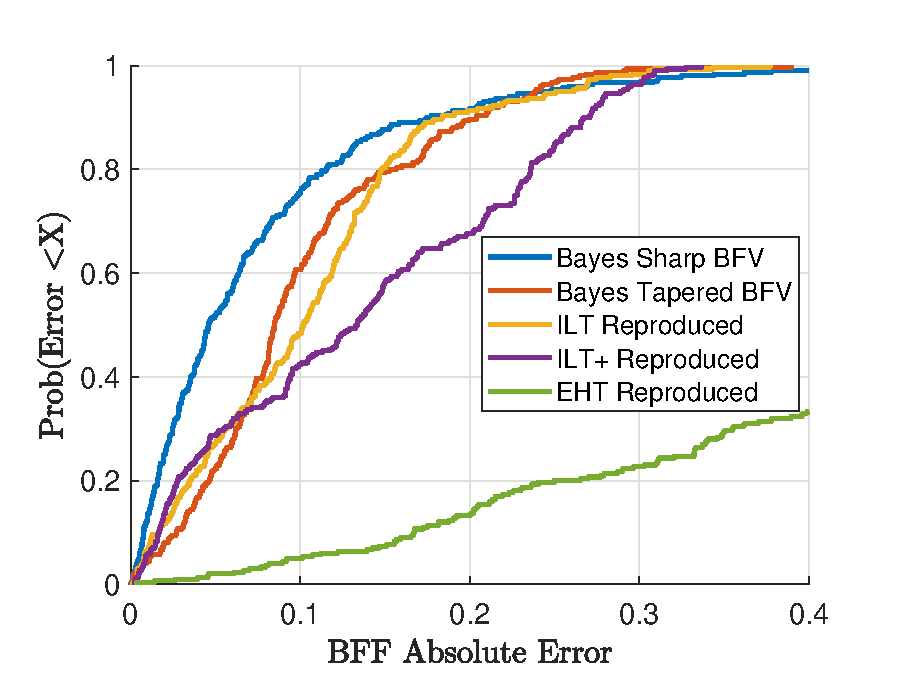
\includegraphics[width = \textwidth]{evaluation/cdf_SNR_1.eps}
        \caption{SNR = 1}
    \end{subfigure}
    \begin{subfigure}[b]{0.49\textwidth}
        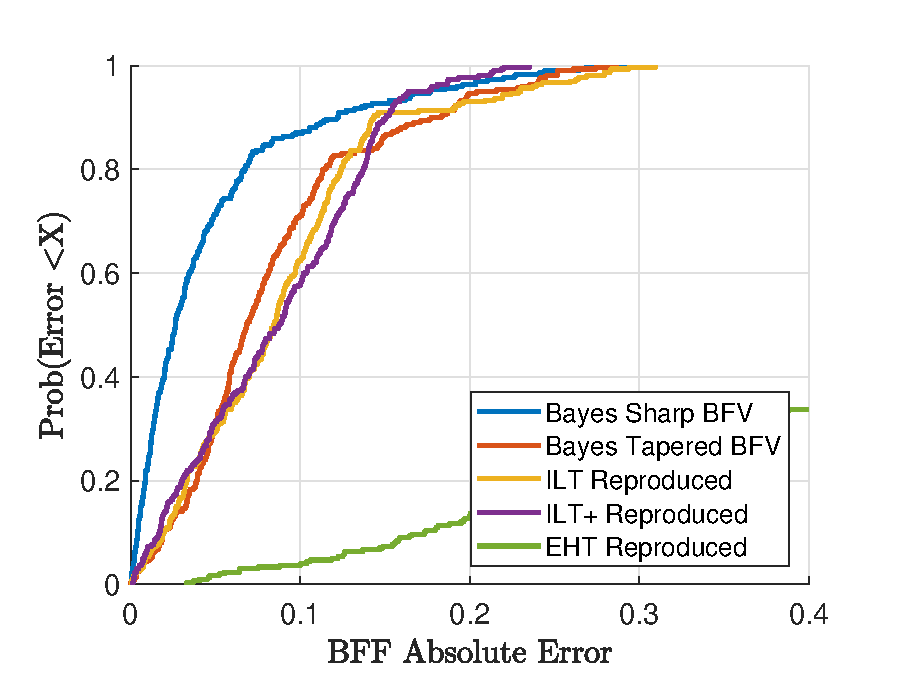
\includegraphics[width = \textwidth]{evaluation/cdf_SNR_5.eps}
        \caption{SNR = 5}
    \end{subfigure}
    \begin{subfigure}[b]{0.49\textwidth}
        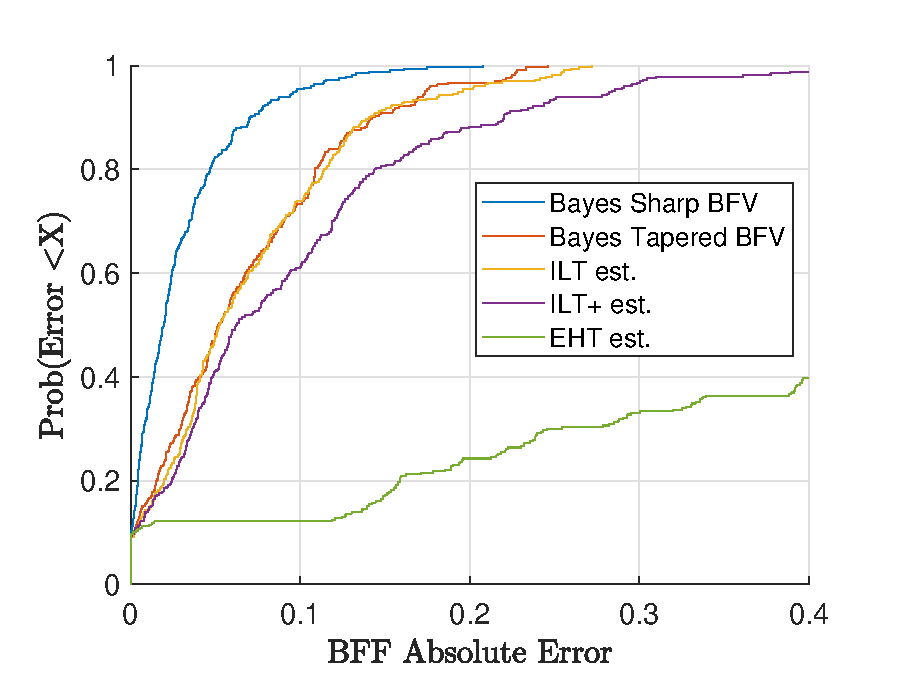
\includegraphics[width = \textwidth]{evaluation/cdf_SNR_10.eps}
        \caption{SNR = 10}
    \end{subfigure}
    \begin{subfigure}[b]{0.49\textwidth}
        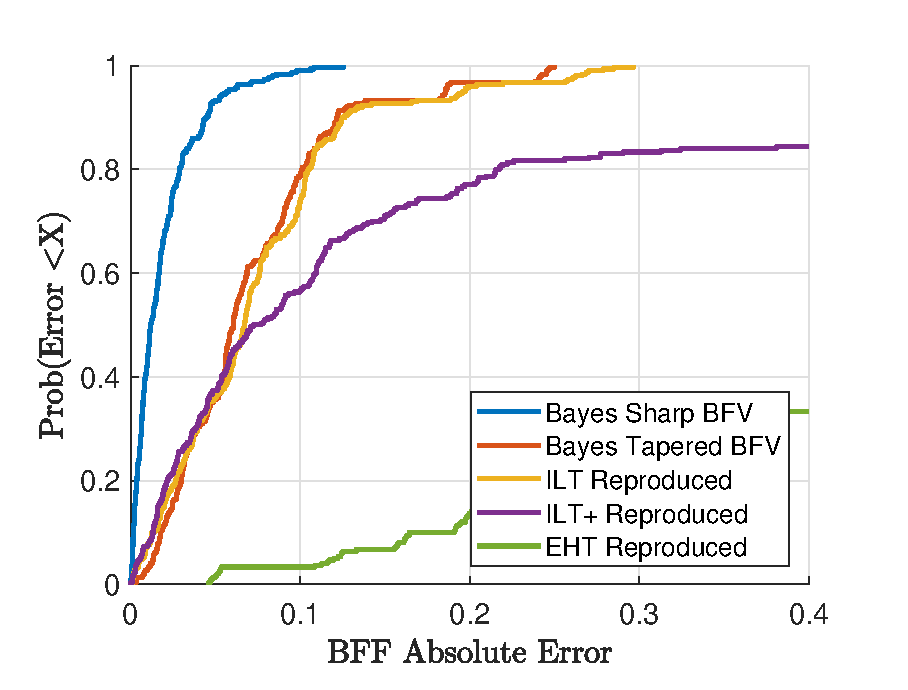
\includegraphics[width = \textwidth]{evaluation/cdf_SNR_100.eps}
        \caption{SNR = 100}
    \end{subfigure}
    \caption{Cumulative distribution functions for BFF estimation error for different SNRs}
    \label{fig:Comparative_SNR}
\end{figure}

\section{Dependence on the Prior}

A crucial element for the Bayesian estimator is its robustness to changes in the prior. Figure \ref{fig:different_prior} compares the BFF estimate absolute error for different amounts of randomly chosen density functions used to construct the prior. We explore the Bayesian estimator with a sharp BFV integral in this analysis. This was repeated via cross-validation for each of the 30 samples 50 times.

This analysis of prior generality illuminates the importance of an effective prior for the Bayesian estimator. As we increase the number of instances that make up the prior, we converge towards a performance bound with diminishing returns. The benefits of an increase to a prior's sample size is pronounced for an increase from 5 to 10 density functions. 50\% of the absolute error is below 0.070 for a prior built from 5 instances. The prior constructed with 10 experimental instances has 50\% of the absolute error below 0.029. This decrease of error by 58\% at this cumulative probability emphasises how a more detailed prior is important for the Bayesian estimator.

The reproduced ILT+, the best of the existing reproduced techniques, tends to generally outperform the Bayesian estimator for where there are 5 or less experimental density functions forming the prior. As the sample size decreases, the Bayesian technique becomes progressively worst as it loses generality. In addition, the Gaussian assumption of the prior density function is less reasonable at these small sample sizes. This exemplifies the Bayesian framework's limitations for generality for where there is little experimental data to form the prior.

\begin{figure}[htb!]
    \centering
    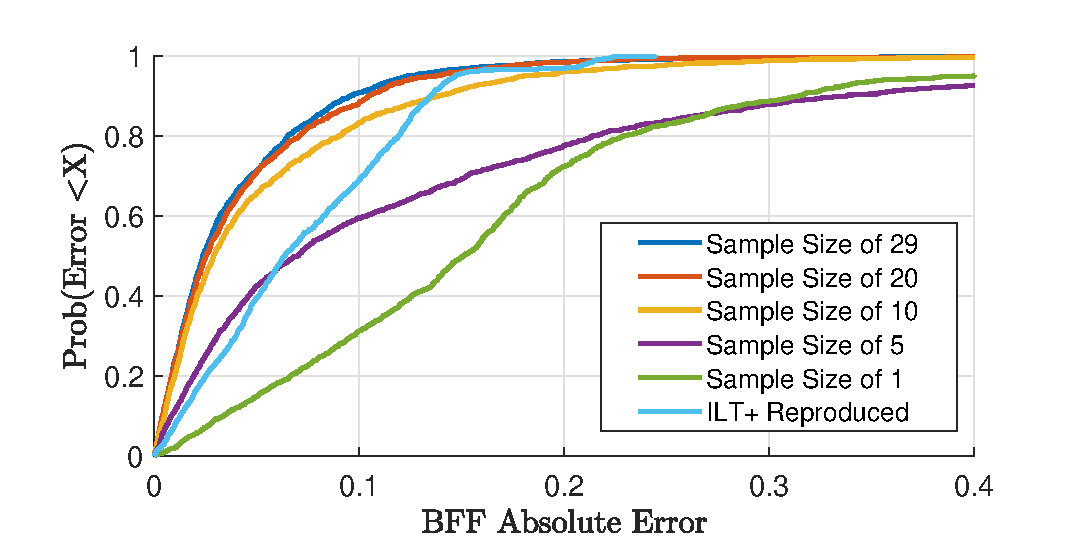
\includegraphics[width=\textwidth]{evaluation/different_priors.eps}
    \caption{CDF comparison of Bayesian estimation absolute error for different numbers of randomly chosen instances forming the prior}
    \label{fig:different_prior}
\end{figure}

\section{Computation Comparison}
Figure \ref{fig:computation_time_results} demonstrates the difference in computation time for each of the techniques. Generally, we see that the proposed Bayesian techniques takes consistently longer than all of the other techniques due to the absence of compressive preprocessing.

The EHT outperforms all of the other techniques, as it requires no matrix inversion or any iterative computation. This comes at the trade off in terms of actual accuracy as demonstrated in Sections \ref{section:aChosenTc_evaluation} - \ref{section:differentSNR_evaluation}. This means it is served best augmenting another method such as the ILT+ rather than being its own standalone estimator.

The ILT and ILT+ are comparable as they contain the intensive singular value decomposition of (\ref{eq:compressedMeasurement}) and multiple matrix inversions of the compressed matrix in (\ref{eq:optFindC}). A matrix inversion has a high computational complexity \cite{invertMatrixComputational}, so if the dimensionality is reduced significantly, performance is decisively increased.

The Bayes method is the slowest as even though there is no iterative computation, it involves the inversion of a term that contains the uncompressed kernel (\ref{eq:posteriorProbability}). This expensive computation implies that compressing the input in some way before introducing it into the framework potentially would yield a better computation speed.


\begin{figure}
    \centering
    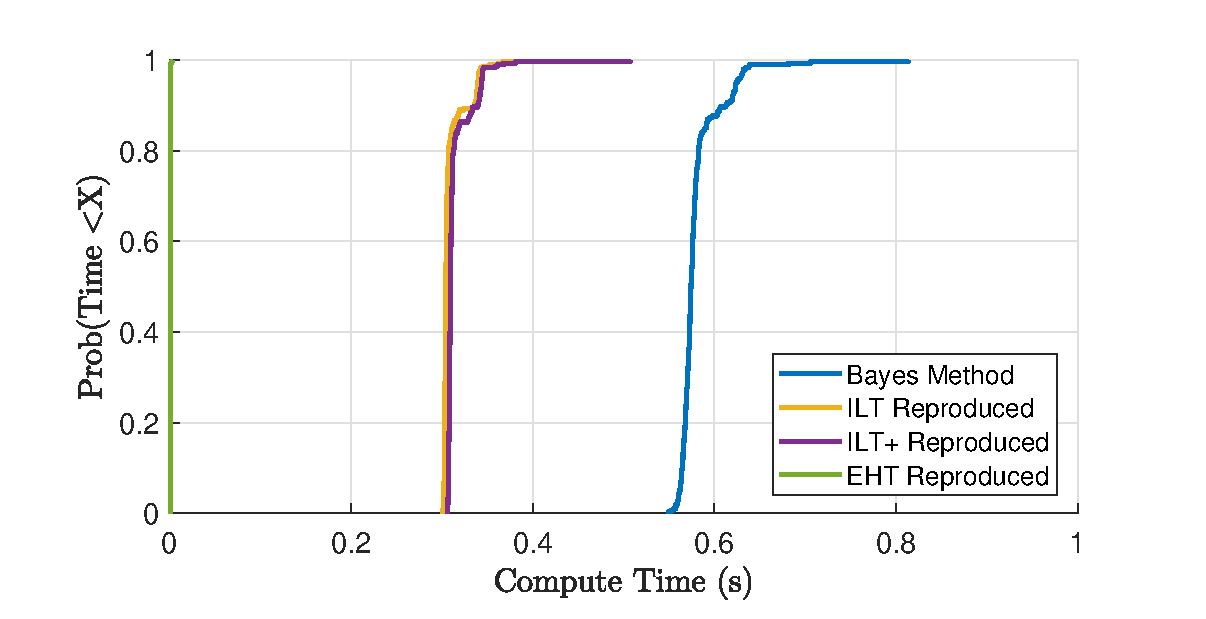
\includegraphics[width = 0.8\textwidth]{evaluation/compute_time_compare.eps}
    \caption{Cumulative distribution functions of computation times for each of the techniques}
    \label{fig:computation_time_results}
\end{figure}

\iffalse
\begin{table}[]
\centering
\begin{tabular}{l c c c c}
\toprule
                      & EHT       & ILT    & ILT+   & Bayes  \\ 
\midrule
Median Time (seconds) & 7.881E-04 & 0.3041 & 0.3093 & 0.5741 \\
\bottomrule
\end{tabular}
\caption{Computation time statistics for the different estimation techniques}
\label{tab:computationTimes}
\end{table}
\fi

\section{Evaluation Conclusions}
We have determined that given a prior that is representative of what is being estimated, we may estimate the BFF more accurately with the Bayesian estimator. This has been demonstrated for different SNR and different bound volume cut-off times ($T_c$). However, it is outperformed in terms of computation due to the lack of compression in the framework and is heavily dependent on its prior. Given that experimental data may be available for potential users of this estimator, the latter is less of a concern. The actual performance of the Bayesian technique for these different performance metrics forms a strong case for its viability and use.


\chapter{Conclusions}\label{C:conclusions}

The project aimed to implement and evaluate the proposed Bayesian estimator alongside the existing published techniques.

In the background, the physical model of NMR relaxation was established. Building off this model, the literature provides a comprehensive benchmark of the current field of estimating T2 relaxation. Satisfying constraints of prior information such as the non-negativity of T2 relaxation times and knowledge of the SNR, they provided robust methods of approximating T2 relaxation density. In nosier environments however, these priori were less useful. An inclusion of a more useful prior grounded in the physical model was required.

The design discusses the how a more useful prior may be implemented with a Bayesian framework. To use a multivariate case of Bayes' theorem such that the it were analytically tractable we assume T2 relaxation timess are to be from a Gaussian distribution. Given this assumption, there is the design question in how we derive the mean and covariance of the prior density function. Allowing for dependence between each of the T2 relaxation bins, at the risk of losing some generality, solves this question. With high quality experimental data embedded into the estimator, we could implement the Bayesian estimator.

Implementation of the existing methods and the proposed method allows for evaluation for different environments such that algorithm robustness and accuracy could be compared. The validation framework built for implementation compares the reproduced and published techniques. The complexity of the ILT+ algorithm complicated direct one-to-one recreation so the reproduction utilised a tuned variation of this. This preserved the indicative performance of the system so that comparison and analysis would be valid. In addition, the proposed Bayesian estimator demonstrated considerable simplicity in implementation in comparison to the majority of the published techniques.

The evaluation of the estimator for different environments in comparison with the reproduced techniques demonstrates the improvements made by using a more comprehensive prior. The Bayesian estimator outperforms the existing reproduced techniques generally for different SNR and bound fluid cut-off. This is done via cross-validation so that we could ensure generality of performance measurement. However, the framework fails if the prior poorly describes what it estimates. With these different perspectives of analysis, we determine that the Bayesian estimator is superior if it has a prior representative of what is measured.

\section{Future Work}
The potential and viability found with the Bayesian framework introduces a potential for its application in other adversely noisy estimation problems. The main parts of this include adapting the Bayesian framework towards different models.

Specifically, additional potential avenues of future work for the Bayes estimator include:
\begin{itemize}
    \item Increasing the computational speed of the estimator. There may be potential in adding compressive technologies to get the full benefit of the non-iterative analytic Bayesian expression.
    \item Examining sensitivity for what forms the prior information, i.e. how well a prior made from only carbonate rock samples may be applicable to sandstone rock samples. 
    \item Can a log-normal noise model be applicable to a tractable Bayesian framework to prevent non-negative density functions.
    \item Could the Bayes framework augment the ILT+ technique to acquire a general and robust estimator with built in flexibility in prior information.
\end{itemize}





%%%%%%%%%%%%%%%%%%%%%%%%%%%%%%%%%%%%%%%%%%%%%%%%%%%%%%%

\backmatter

%%%%%%%%%%%%%%%%%%%%%%%%%%%%%%%%%%%%%%%%%%%%%%%%%%%%%%%


\bibliographystyle{ieeetr}
%\bibliographystyle{acm}
\bibliography{sample}

\chapter{Appendix}
\section{Meeting Notes}
\includepdf[pages=-]{meeting_notes.pdf}


\end{document}
